%%%%%%%%%%%%%%%%%%%%%%%%%%%%%%%%%%%%%%%%%%%%%%%%%%%%%%%%%%%%%%%%%%%%%%%%%%%%%%%
% Net Zero Pathways for Korea's Petrochemical Industry
% A Facility-Level Marginal Abatement Cost Analysis
% PLANiT Institute, 2025
%%%%%%%%%%%%%%%%%%%%%%%%%%%%%%%%%%%%%%%%%%%%%%%%%%%%%%%%%%%%%%%%%%%%%%%%%%%%%%%

\documentclass[12pt,a4paper]{article}

%% Encoding and Fonts
\usepackage[utf8]{inputenc}
\usepackage[T1]{fontenc}
\usepackage{lmodern}

%% Mathematics
\usepackage{amsmath,amssymb,amsfonts}

%% Graphics and Figures
\usepackage{graphicx}
\usepackage{float}
\usepackage{caption}
\usepackage{subcaption}

%% Tables
\usepackage{booktabs}
\usepackage{multirow}
\usepackage{array}
\usepackage{longtable}
\usepackage{tabularx}

%% Units and Numbers
\usepackage{siunitx}
\sisetup{
  group-separator = {,},
  group-minimum-digits = 4,
  detect-all
}

%% Page Layout
\usepackage[margin=2.5cm]{geometry}
\usepackage{setspace}
\onehalfspacing
\setlength{\parindent}{0pt}
\setlength{\parskip}{6pt}
\setlength{\headheight}{14pt}

%% Colors
\usepackage[table]{xcolor}
\definecolor{tableheader}{RGB}{240,240,240}
\definecolor{linkblue}{RGB}{0,0,139}

%% Hyperlinks
\usepackage[colorlinks=true,linkcolor=linkblue,citecolor=linkblue,urlcolor=linkblue]{hyperref}

%% Bibliography
\usepackage[authoryear,round]{natbib}
\bibliographystyle{apalike}

%% Landscape pages
\usepackage{pdflscape}

%% Header/Footer
\usepackage{fancyhdr}
\pagestyle{fancy}
\fancyhf{}
\rhead{\small PLANiT Institute}
\lhead{\small Petrochemical Decarbonization Analysis}
\cfoot{\thepage}

%% Custom commands
\newcommand{\COtwo}{CO\textsubscript{2}}
\newcommand{\HTwo}{H\textsubscript{2}}
\newcommand{\mtco}{Mt~\COtwo}
\newcommand{\tco}{t~\COtwo}
\newcommand{\usdperton}{\$/t~\COtwo}

%%%%%%%%%%%%%%%%%%%%%%%%%%%%%%%%%%%%%%%%%%%%%%%%%%%%%%%%%%%%%%%%%%%%%%%%%%%%%%%
\begin{document}

%% Title Page
\begin{titlepage}
\centering
\vspace*{2cm}

{\LARGE\bfseries Net Zero Pathways for Korea's Petrochemical Industry}\\[0.5cm]
{\Large A Facility-Level Marginal Abatement Cost Analysis}\\[2cm]

{\large PLANiT Institute}\\
{\normalsize Seoul, Republic of Korea}\\[1cm]

{\large Technical Report}\\[0.5cm]
{\normalsize Version 1.0}\\[2cm]

{\large January 2026}\\[3cm]

\vfill
{\small
\textbf{Corresponding Author:}\\
PLANiT Institute\\
Seoul, Republic of Korea\\
\texttt{research@planit.re.kr}
}

\end{titlepage}

%%%%%%%%%%%%%%%%%%%%%%%%%%%%%%%%%%%%%%%%%%%%%%%%%%%%%%%%%%%%%%%%%%%%%%%%%%%%%%%
%% Abstract
%%%%%%%%%%%%%%%%%%%%%%%%%%%%%%%%%%%%%%%%%%%%%%%%%%%%%%%%%%%%%%%%%%%%%%%%%%%%%%%
\newpage
\section*{Abstract}

This study presents a comprehensive facility-level analysis of decarbonization pathways for Korea's petrochemical industry, one of the nation's largest industrial emitters. Using a bottom-up marginal abatement cost curve (MACC) approach, we model 237--243 production facilities across four major petrochemical complexes (Yeosu, Daesan, Ulsan, and other sites) under six distinct scenarios combining three production pathways with two technology options.

The baseline analysis reveals total industry emissions of approximately \SI{59.2}{Mt~\COtwo/year} at 70\% operating capacity, concentrated among four major companies (LG Chem, Lotte Chemical, Yeochon NCC, and Hanwha TotalEnergies) that account for 53\% of sectoral emissions. The Yeosu complex alone contributes 38\% of total emissions, followed by Daesan (29\%) and Ulsan (25\%).

We evaluate two primary decarbonization technologies for naphtha cracking furnaces: hydrogen-based combustion (NCC-H2) and electric furnaces (NCC-Electricity), both available from 2030, alongside heat pumps for low-temperature processes (available 2025) and rotodynamic heaters for BTX plants (available 2026). Technology cost assumptions follow a 50\% CAPEX reduction trajectory from 2025 to 2050, consistent with learning curve projections from IRENA and IEA.

Key findings include:

\begin{enumerate}
\item All six scenarios achieve net-zero emissions by 2050 through optimized technology deployment.
\item Cumulative capital expenditure ranges from \$113.5 billion (40\% restructuring with H2) to \$1,242 billion (Shaheen expansion with electricity), demonstrating that production pathway choices have greater cost implications than technology selection.
\item Restructuring scenarios that retire 25--40\% of the oldest naphtha cracker capacity reduce cumulative CAPEX by 85--91\% compared to growth scenarios.
\item Hydrogen-based scenarios consistently show lower cumulative CAPEX (\$113--826 billion) than electric alternatives (\$115--1,242 billion), though electric pathways may achieve negative net operating costs due to fuel savings.
\item Under a 1.5°C-aligned carbon budget, stranded asset exposure ranges from \$14.4 billion to \$24.6 billion, with earlier stranding years (2028--2032) requiring accelerated technology deployment.
\item Final-year electricity demand ranges from 18.5 to 273.6 TWh, while hydrogen demand reaches 2.0--4.3 Mt for H2-based scenarios, implying substantial renewable energy infrastructure requirements of 5--85 GW equivalent capacity.
\end{enumerate}

The analysis demonstrates that Korea's petrochemical industry can technically achieve net-zero emissions by 2050 under all evaluated scenarios, but the choice between capacity growth versus restructuring has profound implications for transition costs, stranded asset risk, and infrastructure requirements. Policy recommendations include prioritizing 25--40\% capacity restructuring to manage costs, developing dedicated hydrogen infrastructure, and aligning carbon pricing with the 2.0°C pathway given technology availability constraints that make the 1.5°C pathway structurally challenging before 2030.

\vspace{0.5cm}
\textbf{Keywords:} Petrochemical industry; Decarbonization; Marginal abatement cost curve; Net zero; Electrification; Green hydrogen; Korea; Climate policy; Stranded assets

%%%%%%%%%%%%%%%%%%%%%%%%%%%%%%%%%%%%%%%%%%%%%%%%%%%%%%%%%%%%%%%%%%%%%%%%%%%%%%%
%% Table of Contents
%%%%%%%%%%%%%%%%%%%%%%%%%%%%%%%%%%%%%%%%%%%%%%%%%%%%%%%%%%%%%%%%%%%%%%%%%%%%%%%
\newpage
\tableofcontents
\newpage

%%%%%%%%%%%%%%%%%%%%%%%%%%%%%%%%%%%%%%%%%%%%%%%%%%%%%%%%%%%%%%%%%%%%%%%%%%%%%%%
%% 1. Introduction
%%%%%%%%%%%%%%%%%%%%%%%%%%%%%%%%%%%%%%%%%%%%%%%%%%%%%%%%%%%%%%%%%%%%%%%%%%%%%%%
\section{Introduction}

\subsection{Background and Motivation}

Korea's petrochemical industry represents one of the nation's most energy-intensive and emission-intensive industrial sectors. With total greenhouse gas emissions of approximately \SI{78}{Mt~\COtwo} annually when accounting for upstream processes and utilities, the sector contributes significantly to Korea's industrial carbon footprint \citep{kpia2024}. This emission intensity, combined with the industry's strategic economic importance---employing over 40,000 workers and generating exports exceeding \$50 billion annually---presents a complex challenge for national decarbonization efforts \citep{motie2023}.

The petrochemical sector's emissions profile is dominated by naphtha steam cracking, which accounts for approximately 70\% of sectoral emissions through high-temperature furnace operations \citep{iea2018}. The remaining emissions arise from auxiliary processes, electricity consumption, and various fuel combustion activities across aromatics (BTX) plants, polymerization units, and utility systems.

Recent developments have intensified the urgency of petrochemical decarbonization. The Korean government's commitment to carbon neutrality by 2050, combined with increasing carbon costs under the Korean Emissions Trading Scheme (K-ETS), creates both regulatory pressure and economic incentive for emission reductions \citep{motie2023}. Simultaneously, accumulated financial losses among major petrochemical companies over recent years have prompted discussions of industry restructuring, potentially offering an opportunity to align capacity rationalization with decarbonization objectives.

\subsection{Research Questions}

This study addresses four primary research questions:

\begin{enumerate}
\item \textbf{Renewable Energy Requirements:} What scale of renewable electricity and green hydrogen infrastructure is required for the petrochemical industry to meet various carbon budget scenarios?

\item \textbf{Technology Costs:} What are the comparative costs and deployment timelines of emerging decarbonization technologies, particularly electric furnaces versus hydrogen-based combustion systems?

\item \textbf{Company-Level Impacts:} What are the transition costs, stranded asset exposures, and renewable energy requirements for individual companies across Korea's major petrochemical complexes?

\item \textbf{Pathway Feasibility:} Which carbon budget pathways (1.5°C, 2.0°C, or NDC-aligned) are technically achievable given technology readiness constraints, and what are the implications for policy design?
\end{enumerate}

\subsection{Contribution and Scope}

This analysis contributes to the existing literature in several ways. First, we develop a comprehensive facility-level database covering 237--243 production units across Korea's petrochemical sector, enabling granular assessment of abatement opportunities and costs. Second, we apply a marginal abatement cost curve (MACC) methodology that accounts for technology availability constraints, learning curve effects, and regional infrastructure considerations. Third, we evaluate multiple production pathway scenarios---including industry restructuring options currently under policy discussion---alongside technology choice dimensions.

The study scope encompasses all major petrochemical products from naphtha cracking (ethylene, propylene, butadiene), aromatics production (benzene, toluene, xylene), and downstream derivatives. The analysis period spans 2025--2050, with annual resolution for emission trajectories, technology deployment, and cost accounting.

%%%%%%%%%%%%%%%%%%%%%%%%%%%%%%%%%%%%%%%%%%%%%%%%%%%%%%%%%%%%%%%%%%%%%%%%%%%%%%%
%% 2. Methodology
%%%%%%%%%%%%%%%%%%%%%%%%%%%%%%%%%%%%%%%%%%%%%%%%%%%%%%%%%%%%%%%%%%%%%%%%%%%%%%%
\section{Methodology}

\subsection{Data Architecture}

The analysis is built upon a comprehensive facility database encompassing Korea's petrochemical production infrastructure. Data sources include:

\begin{itemize}
\item Korea Petrochemical Industry Association (KPIA) production statistics \citep{kpia2024}
\item Korea Institute of Energy Research (KIER) energy efficiency benchmarks \citep{kier2022}
\item Company-level disclosures and environmental reports
\item PLANiT Institute internal facility mapping \citep{planit2025}
\end{itemize}

The database includes 237 baseline facilities (243 including planned Shaheen project additions), with attributes covering product type, process technology, capacity, location, company ownership, construction year, and detailed energy consumption profiles by fuel type.

\subsection{Emission Factor Framework}

Baseline emissions are calculated using fuel-specific emission factors consistent with IPCC guidelines \citep{ipcc2019} and API methodologies \citep{api2021}. Table~\ref{tab:emission_factors} presents the emission factors applied in this analysis.

\begin{table}[H]
\centering
\caption{Combustion Emission Factors by Fuel Type}
\label{tab:emission_factors}
\begin{tabular}{@{}llll@{}}
\toprule
\textbf{Fuel} & \textbf{Emission Factor} & \textbf{Unit} & \textbf{Source} \\
\midrule
Naphtha & 0.0542 & \tco/GJ & IPCC 2019 \\
Electricity (Grid) & 0.436 & \tco/MWh & Korea Grid 2025 \\
LNG & 0.0561 & \tco/GJ & IPCC 2019 \\
Fuel Gas & 0.050 & \tco/GJ & API 2021 \\
Byproduct Gas & 0.048 & \tco/GJ & API 2021 \\
LPG & 0.0631 & \tco/GJ & IPCC 2019 \\
Fuel Oil & 0.0773 & \tco/GJ & IPCC 2019 \\
Diesel & 0.0741 & \tco/GJ & IPCC 2019 \\
Green Hydrogen & 0.0 & \tco/kg & By definition \\
\bottomrule
\end{tabular}
\end{table}

Grid electricity emission factors are assumed to decline linearly from \SI{0.436}{t~\COtwo/MWh} in 2025 to zero by 2050, consistent with Korea's power sector decarbonization targets.

\subsection{Energy Intensity Benchmarks}

Energy consumption is modeled using product-specific intensity benchmarks derived from industry best practices and Korean facility data \citep{saygin2011, kier2022}. Table~\ref{tab:energy_intensity} presents benchmark values for major product categories.

\begin{table}[H]
\centering
\caption{Energy Intensity Benchmarks for Major Products}
\label{tab:energy_intensity}
\begin{tabular}{@{}lrrrl@{}}
\toprule
\textbf{Product} & \textbf{Naphtha} & \textbf{Electricity} & \textbf{LNG} & \textbf{Process} \\
 & (GJ/t) & (kWh/t) & (GJ/t) & \\
\midrule
Ethylene & 29.00 & 85.42 & 2.03 & Naphtha Cracker \\
Propylene & 25.39 & 191.27 & 1.78 & Naphtha Cracker \\
Butadiene & 29.00 & 400.04 & 2.03 & Naphtha Cracker \\
Benzene & --- & 36.60 & 1.15 & BTX Plant \\
Toluene & --- & 49.53 & 1.68 & BTX Plant \\
Xylene & --- & 763.08 & 1.72 & BTX Plant \\
HDPE & --- & 1,370.60 & --- & Polymerization \\
LDPE & --- & 1,762.00 & --- & Polymerization \\
\bottomrule
\end{tabular}
\end{table}

\subsection{Marginal Abatement Cost Methodology}

The marginal abatement cost (MAC) for each technology-facility combination is calculated as:

\begin{equation}
\text{MAC} = \frac{\text{CAPEX}_{\text{annual}} + \text{OPEX} + \text{New Energy Cost} - \text{Fuel Savings}}{\text{Abatement Potential}}
\label{eq:mac}
\end{equation}

where CAPEX$_{\text{annual}}$ represents annualized capital expenditure over the technology lifetime, and abatement potential is calculated based on the emissions displaced by the new technology.

For inter-temporal optimization across the 2025--2050 analysis period, we employ the Levelized Cost of Abatement (LCOA):

\begin{equation}
\text{LCOA} = \frac{\sum_{t=2025}^{2050} \frac{\text{Annual Cost}_t}{(1+r)^{t-2025}}}{\sum_{t=2025}^{2050} \text{Abatement}_t}
\label{eq:lcoa}
\end{equation}

where $r = 0.08$ (8\% discount rate) represents the weighted average cost of capital for industrial investments.

\subsection{Levelized Cost of Hydrogen}

Green hydrogen costs are modeled using a bottom-up levelized cost methodology:

\begin{equation}
\text{LCOH} = \frac{\text{Electrolyzer CAPEX} \times \text{CRF} + \text{O\&M}}{\text{Annual H}_2\text{ Production}} + \frac{\text{Electricity Cost}}{\text{Electrolyzer Efficiency}}
\label{eq:lcoh}
\end{equation}

where the Capital Recovery Factor (CRF) converts overnight capital costs to annual payments over the assumed 20-year electrolyzer lifetime. Key assumptions for LCOH calculation are presented in Table~\ref{tab:lcoh_assumptions}.

\begin{table}[H]
\centering
\caption{Levelized Cost of Hydrogen Calculation Assumptions}
\label{tab:lcoh_assumptions}
\begin{tabular}{@{}lrrrrr@{}}
\toprule
\textbf{Parameter} & \textbf{2025} & \textbf{2030} & \textbf{2040} & \textbf{2050} & \textbf{Unit} \\
\midrule
Electrolyzer CAPEX & 1,000 & 900 & 700 & 500 & \$/kW \\
Efficiency & 70 & 71 & 73 & 75 & \% \\
RE-PPA Price & 65 & 55.7 & 40.9 & 30.0 & \$/MWh \\
Resulting LCOH & 4.58 & 3.91 & 2.82 & 2.01 & \$/kg \\
\bottomrule
\end{tabular}
\end{table}

\subsection{Optimization Model Formulation}

The deployment model minimizes total system abatement cost subject to annual emission constraints. The objective function is:

\begin{equation}
\min_{x_{i,t}} \sum_{t=2025}^{2050} \sum_{i \in \mathcal{F}} \text{LCOA}_{i,t} \cdot x_{i,t}
\label{eq:objective}
\end{equation}

subject to:

\begin{align}
\sum_{i \in \mathcal{F}} E_{i,t} \cdot (1 - x_{i,t} \cdot \eta_i) &\leq B_t & \forall t \label{eq:emission_constraint}\\
x_{i,t} &\leq A_{i,t} & \forall i, t \label{eq:availability}\\
x_{i,t} &\in \{0, 1\} & \forall i, t \label{eq:binary}\\
x_{i,t} &\leq x_{i,t+1} & \forall i, t < 2050 \label{eq:irreversibility}
\end{align}

where:
\begin{itemize}
\item $\mathcal{F}$: Set of all facilities ($|\mathcal{F}| = 237$--243 depending on scenario)
\item $x_{i,t}$: Binary deployment decision for facility $i$ in year $t$
\item $\text{LCOA}_{i,t}$: Levelized Cost of Abatement for facility $i$ (\$/tCO$_2$)
\item $E_{i,t}$: Baseline emissions of facility $i$ in year $t$ (tCO$_2$)
\item $\eta_i$: Abatement efficiency of technology applied to facility $i$ (typically 95--100\%)
\item $B_t$: Carbon budget constraint in year $t$ (tCO$_2$)
\item $A_{i,t}$: Technology availability indicator (0 before availability year, 1 after)
\end{itemize}

Constraint~\eqref{eq:emission_constraint} ensures total emissions remain within the annual carbon budget. Constraint~\eqref{eq:availability} prevents deployment before technologies become available (e.g., NCC technologies from 2030). Constraint~\eqref{eq:irreversibility} enforces that once a facility deploys abatement technology, it remains deployed.

The LCOA calculation incorporates all cost components over the technology lifetime:

\begin{equation}
\text{LCOA}_i = \frac{\sum_{t=t_0}^{T} \frac{C_{i,t}^{\text{tech}} + C_{i,t}^{\text{energy}} - S_{i,t}^{\text{fuel}}}{(1+r)^{t-t_0}}}{\sum_{t=t_0}^{T} A_{i,t}}
\label{eq:lcoa_detailed}
\end{equation}

where $C^{\text{tech}}$ is annualized technology cost (CAPEX/lifetime + OPEX), $C^{\text{energy}}$ is new energy cost (hydrogen or renewable electricity), $S^{\text{fuel}}$ is fuel savings from displaced fossil fuels, and $r = 0.08$ is the discount rate.

Figure~\ref{fig:data_architecture} illustrates the complete data architecture and model workflow from input data through optimization to output results.

\begin{figure}[H]
\centering
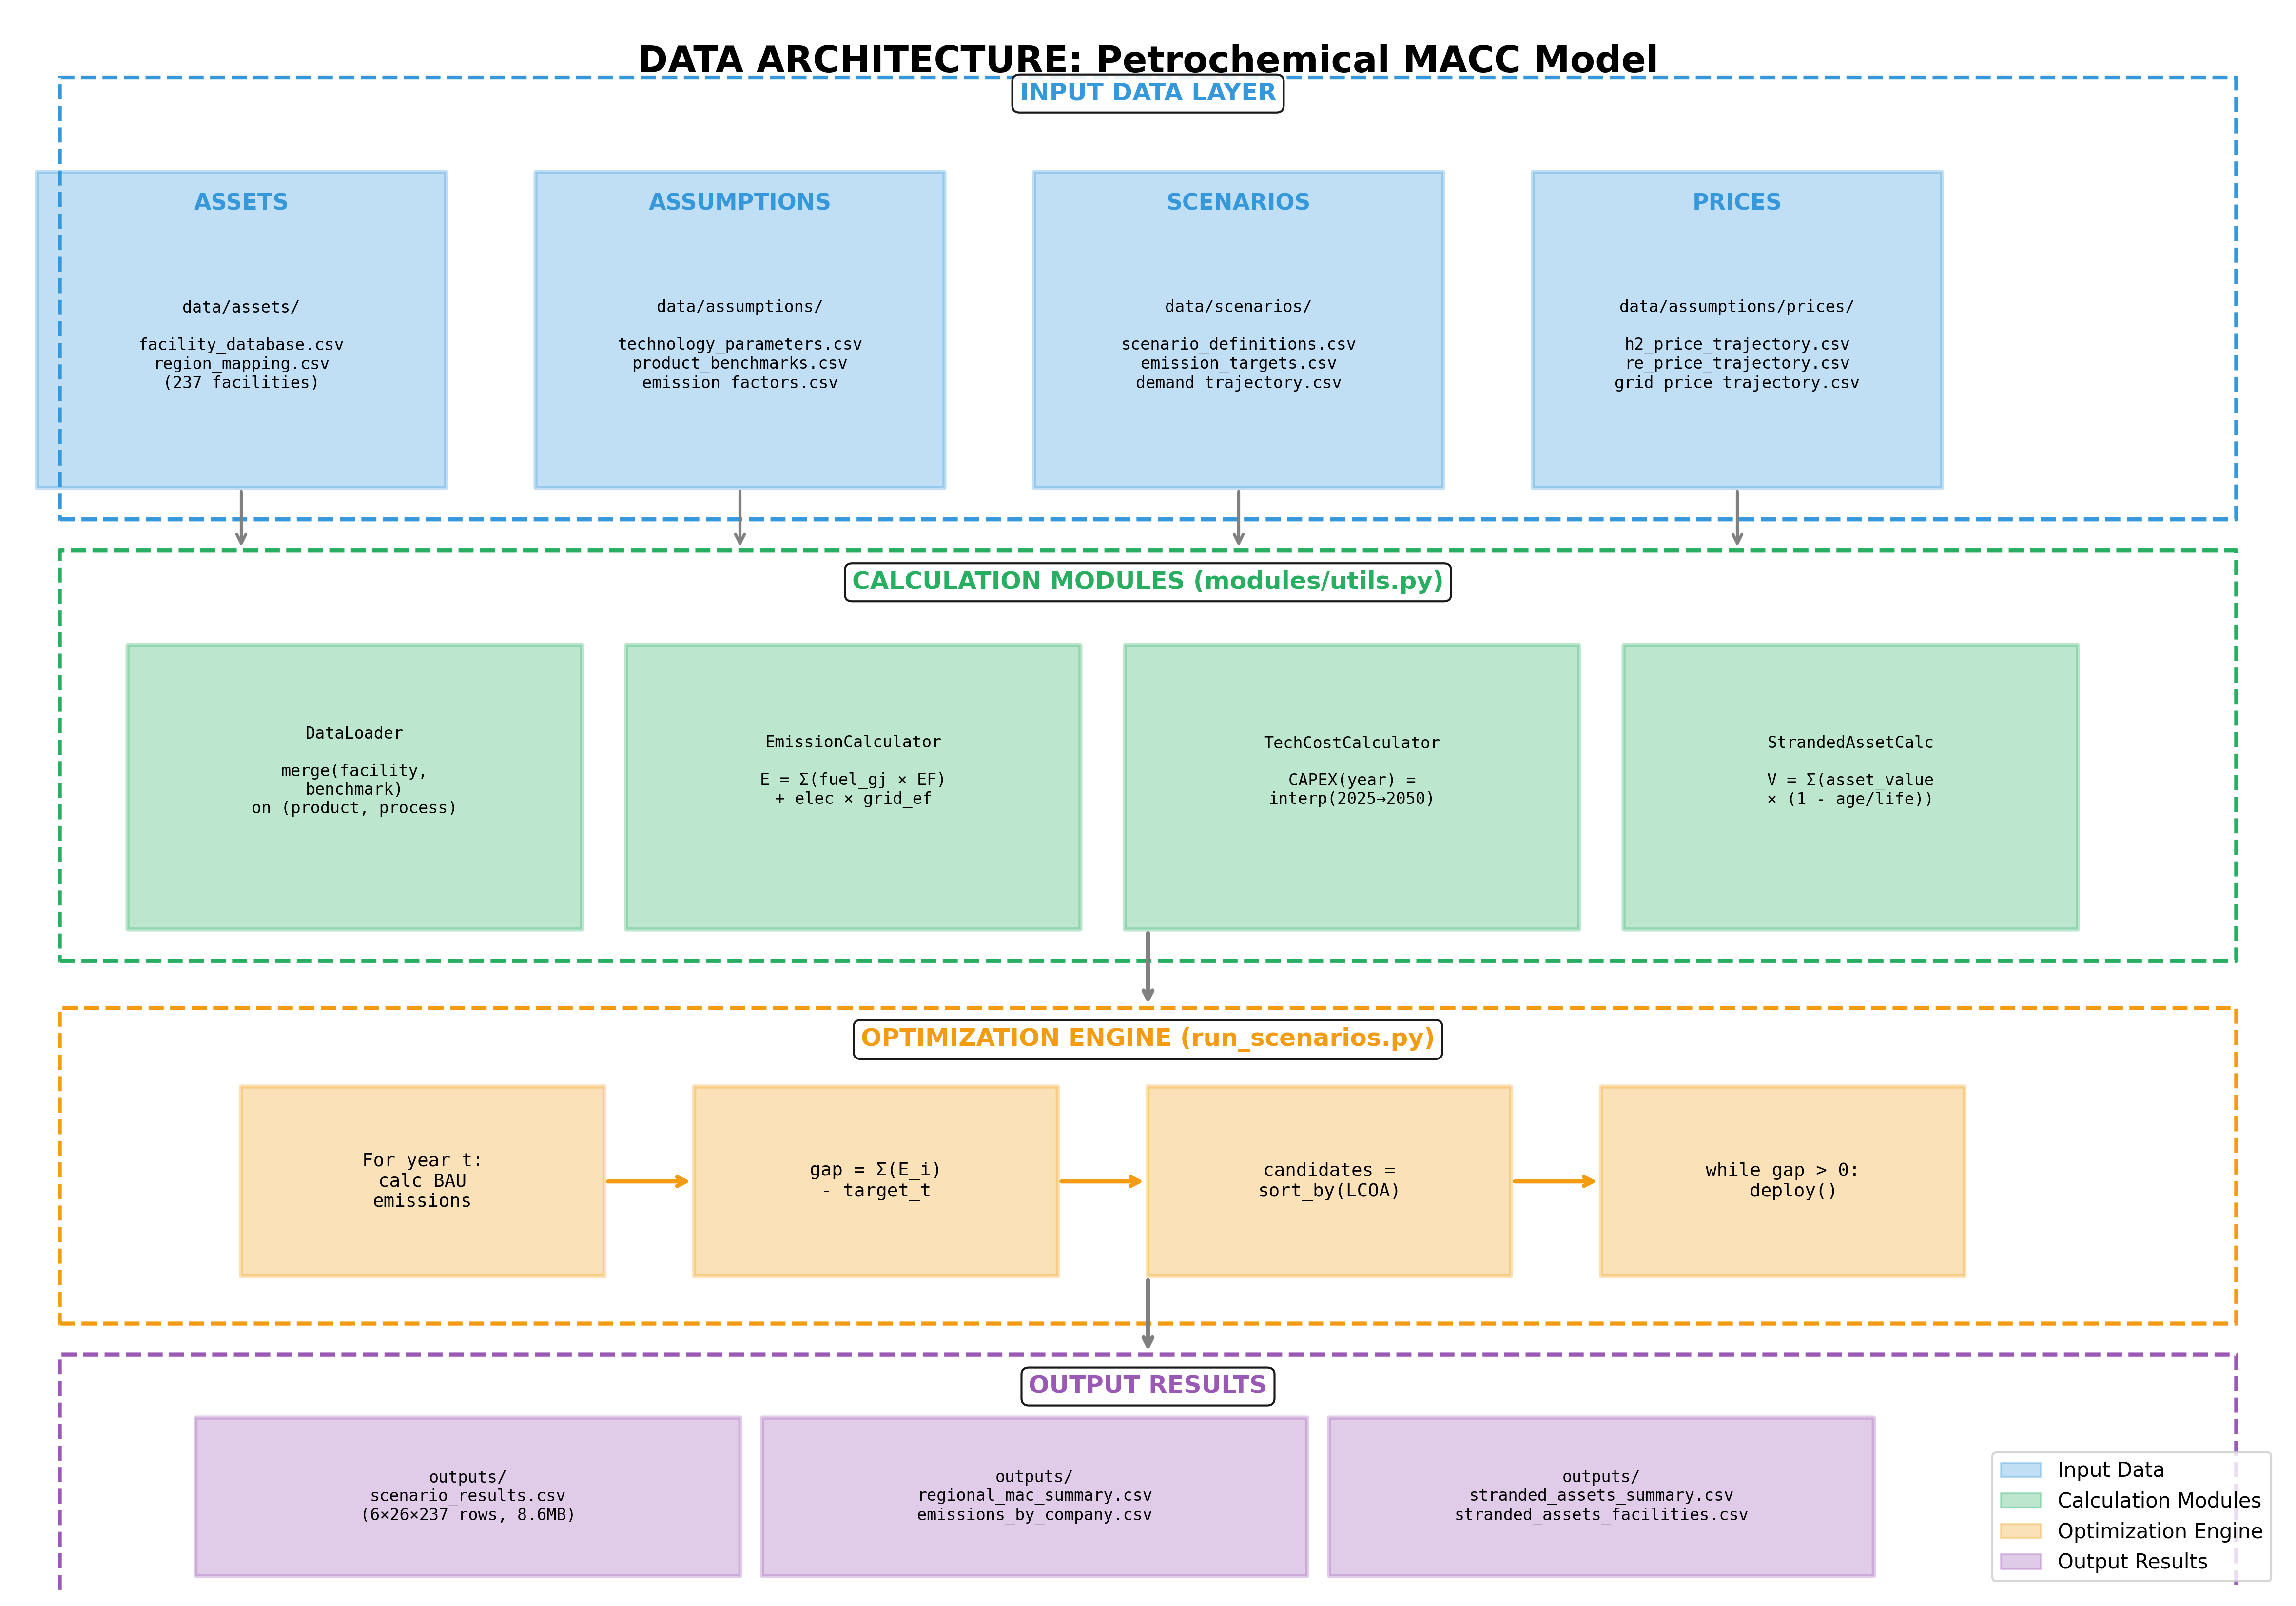
\includegraphics[width=0.95\textwidth]{../outputs/figures/report_data_architecture.png}
\caption{Data architecture and optimization workflow. Input data (blue) flows through calculation modules (green) to the year-by-year optimization engine (orange), producing scenario results (purple). File paths indicate actual CSV data sources.}
\label{fig:data_architecture}
\end{figure}

%%%%%%%%%%%%%%%%%%%%%%%%%%%%%%%%%%%%%%%%%%%%%%%%%%%%%%%%%%%%%%%%%%%%%%%%%%%%%%%
%% 3. Scenario Design
%%%%%%%%%%%%%%%%%%%%%%%%%%%%%%%%%%%%%%%%%%%%%%%%%%%%%%%%%%%%%%%%%%%%%%%%%%%%%%%
\section{Scenario Design}

\subsection{Production Pathway Scenarios}

Three production pathway scenarios are evaluated to capture the range of potential industry trajectories:

\begin{enumerate}
\item \textbf{Shaheen (Growth):} Baseline capacity plus six new S-Oil facilities from 2026, representing continued industry expansion (243 total facilities).

\item \textbf{Restructure 25\%:} Retirement of 25\% of the oldest naphtha cracker capacity, representing moderate industry rationalization (237 facilities with reduced utilization).

\item \textbf{Restructure 40\%:} Retirement of 40\% of the oldest naphtha cracker capacity, representing aggressive restructuring aligned with industry loss mitigation (237 facilities with significantly reduced utilization).
\end{enumerate}

\subsection{Technology Option Scenarios}

Two technology pathways are evaluated for naphtha cracker decarbonization:

\begin{enumerate}
\item \textbf{NCC-H2 (Hydrogen):} Green hydrogen-based combustion replacing naphtha in cracking furnaces, with hydrogen demand of \SI{0.2}{t-\HTwo/t-ethylene} \citep{iea2023hydrogen}.

\item \textbf{NCC-Electricity (Electric):} Electric cracking furnaces based on BASF/SABIC/Linde demonstration technology, with electricity demand of \SI{5.0}{MWh/t-ethylene} \citep{basf2024}.
\end{enumerate}

\subsection{Combined Scenario Matrix}

The combination of three production pathways with two technology options yields six scenarios, summarized in Table~\ref{tab:scenarios}.

\begin{table}[H]
\centering
\caption{Scenario Definitions}
\label{tab:scenarios}
\begin{tabular}{@{}llcl@{}}
\toprule
\textbf{Scenario} & \textbf{Pathway} & \textbf{Facilities} & \textbf{NCC Technology} \\
\midrule
shaheen\_ncc\_h2 & Shaheen (Growth) & 243 & Hydrogen \\
shaheen\_ncc\_elec & Shaheen (Growth) & 243 & Electric \\
restructure\_25pct\_ncc\_h2 & 25\% Restructure & 237 & Hydrogen \\
restructure\_25pct\_ncc\_elec & 25\% Restructure & 237 & Electric \\
restructure\_40pct\_ncc\_h2 & 40\% Restructure & 237 & Hydrogen \\
restructure\_40pct\_ncc\_elec & 40\% Restructure & 237 & Electric \\
\bottomrule
\end{tabular}
\end{table}

\subsection{Carbon Budget Pathways}

Three carbon budget pathways define the emission constraints against which scenarios are evaluated:

\begin{table}[H]
\centering
\caption{Carbon Budget Pathways for Korea's Petrochemical Sector}
\label{tab:carbon_budgets}
\begin{tabular}{@{}lrrr@{}}
\toprule
\textbf{Year} & \textbf{1.5°C} & \textbf{2.0°C} & \textbf{NDC} \\
 & (Mt \COtwo) & (Mt \COtwo) & (Mt \COtwo) \\
\midrule
2025 & 50.0 & 60.0 & 70.0 \\
2030 & 25.0 & 50.0 & 65.0 \\
2035 & 0.0 & 40.0 & 60.0 \\
2040 & 0.0 & 30.0 & 55.0 \\
2045 & 0.0 & 20.0 & 50.0 \\
2050 & 0.0 & 10.0 & 45.0 \\
\bottomrule
\end{tabular}
\end{table}

The 1.5°C pathway requires net-zero by 2035, the 2.0°C pathway targets \SI{10}{Mt~\COtwo} by 2050, and the NDC pathway maintains \SI{45}{Mt~\COtwo} by 2050, consistent with Korea's nationally determined contribution.

%%%%%%%%%%%%%%%%%%%%%%%%%%%%%%%%%%%%%%%%%%%%%%%%%%%%%%%%%%%%%%%%%%%%%%%%%%%%%%%
%% 4. Results
%%%%%%%%%%%%%%%%%%%%%%%%%%%%%%%%%%%%%%%%%%%%%%%%%%%%%%%%%%%%%%%%%%%%%%%%%%%%%%%
\section{Results}

\subsection{Scenario Comparison}

Table~\ref{tab:scenario_results} presents the comprehensive results across all six scenarios, including baseline emissions, cumulative investment, and final-year energy demands.

\begin{table}[H]
\centering
\caption{Scenario Results Summary (2025--2050)}
\label{tab:scenario_results}
\begin{tabular}{@{}lrrrrr@{}}
\toprule
\textbf{Scenario} & \textbf{Baseline} & \textbf{Final} & \textbf{Cum. CAPEX} & \textbf{Elec. 2050} & \textbf{H$_2$ 2050} \\
 & (Mt \COtwo) & (Mt \COtwo) & (\$B) & (TWh) & (Mt) \\
\midrule
shaheen\_ncc\_h2 & 59.25 & 0.0 & 825.87 & 166.43 & 4.28 \\
shaheen\_ncc\_elec & 59.25 & 0.0 & 1,242.06 & 273.58 & 0.00 \\
restructure\_25pct\_ncc\_h2 & 54.81 & 0.0 & 157.68 & 18.49 & 2.33 \\
restructure\_25pct\_ncc\_elec & 54.81 & 0.0 & 160.34 & 76.89 & 0.00 \\
restructure\_40pct\_ncc\_h2 & 54.81 & 0.0 & 113.47 & 40.97 & 2.03 \\
restructure\_40pct\_ncc\_elec & 54.81 & 0.0 & 115.45 & 93.32 & 0.00 \\
\bottomrule
\end{tabular}
\end{table}

All scenarios achieve net-zero emissions by 2050 through optimized technology deployment. However, cumulative CAPEX varies by an order of magnitude, from \$113.5 billion (restructure\_40pct\_ncc\_h2) to \$1,242 billion (shaheen\_ncc\_elec). This variation is driven primarily by the production pathway rather than technology choice.

Figure~\ref{fig:emissions_trajectory} presents the emission trajectories for all six scenarios.

\begin{figure}[H]
\centering
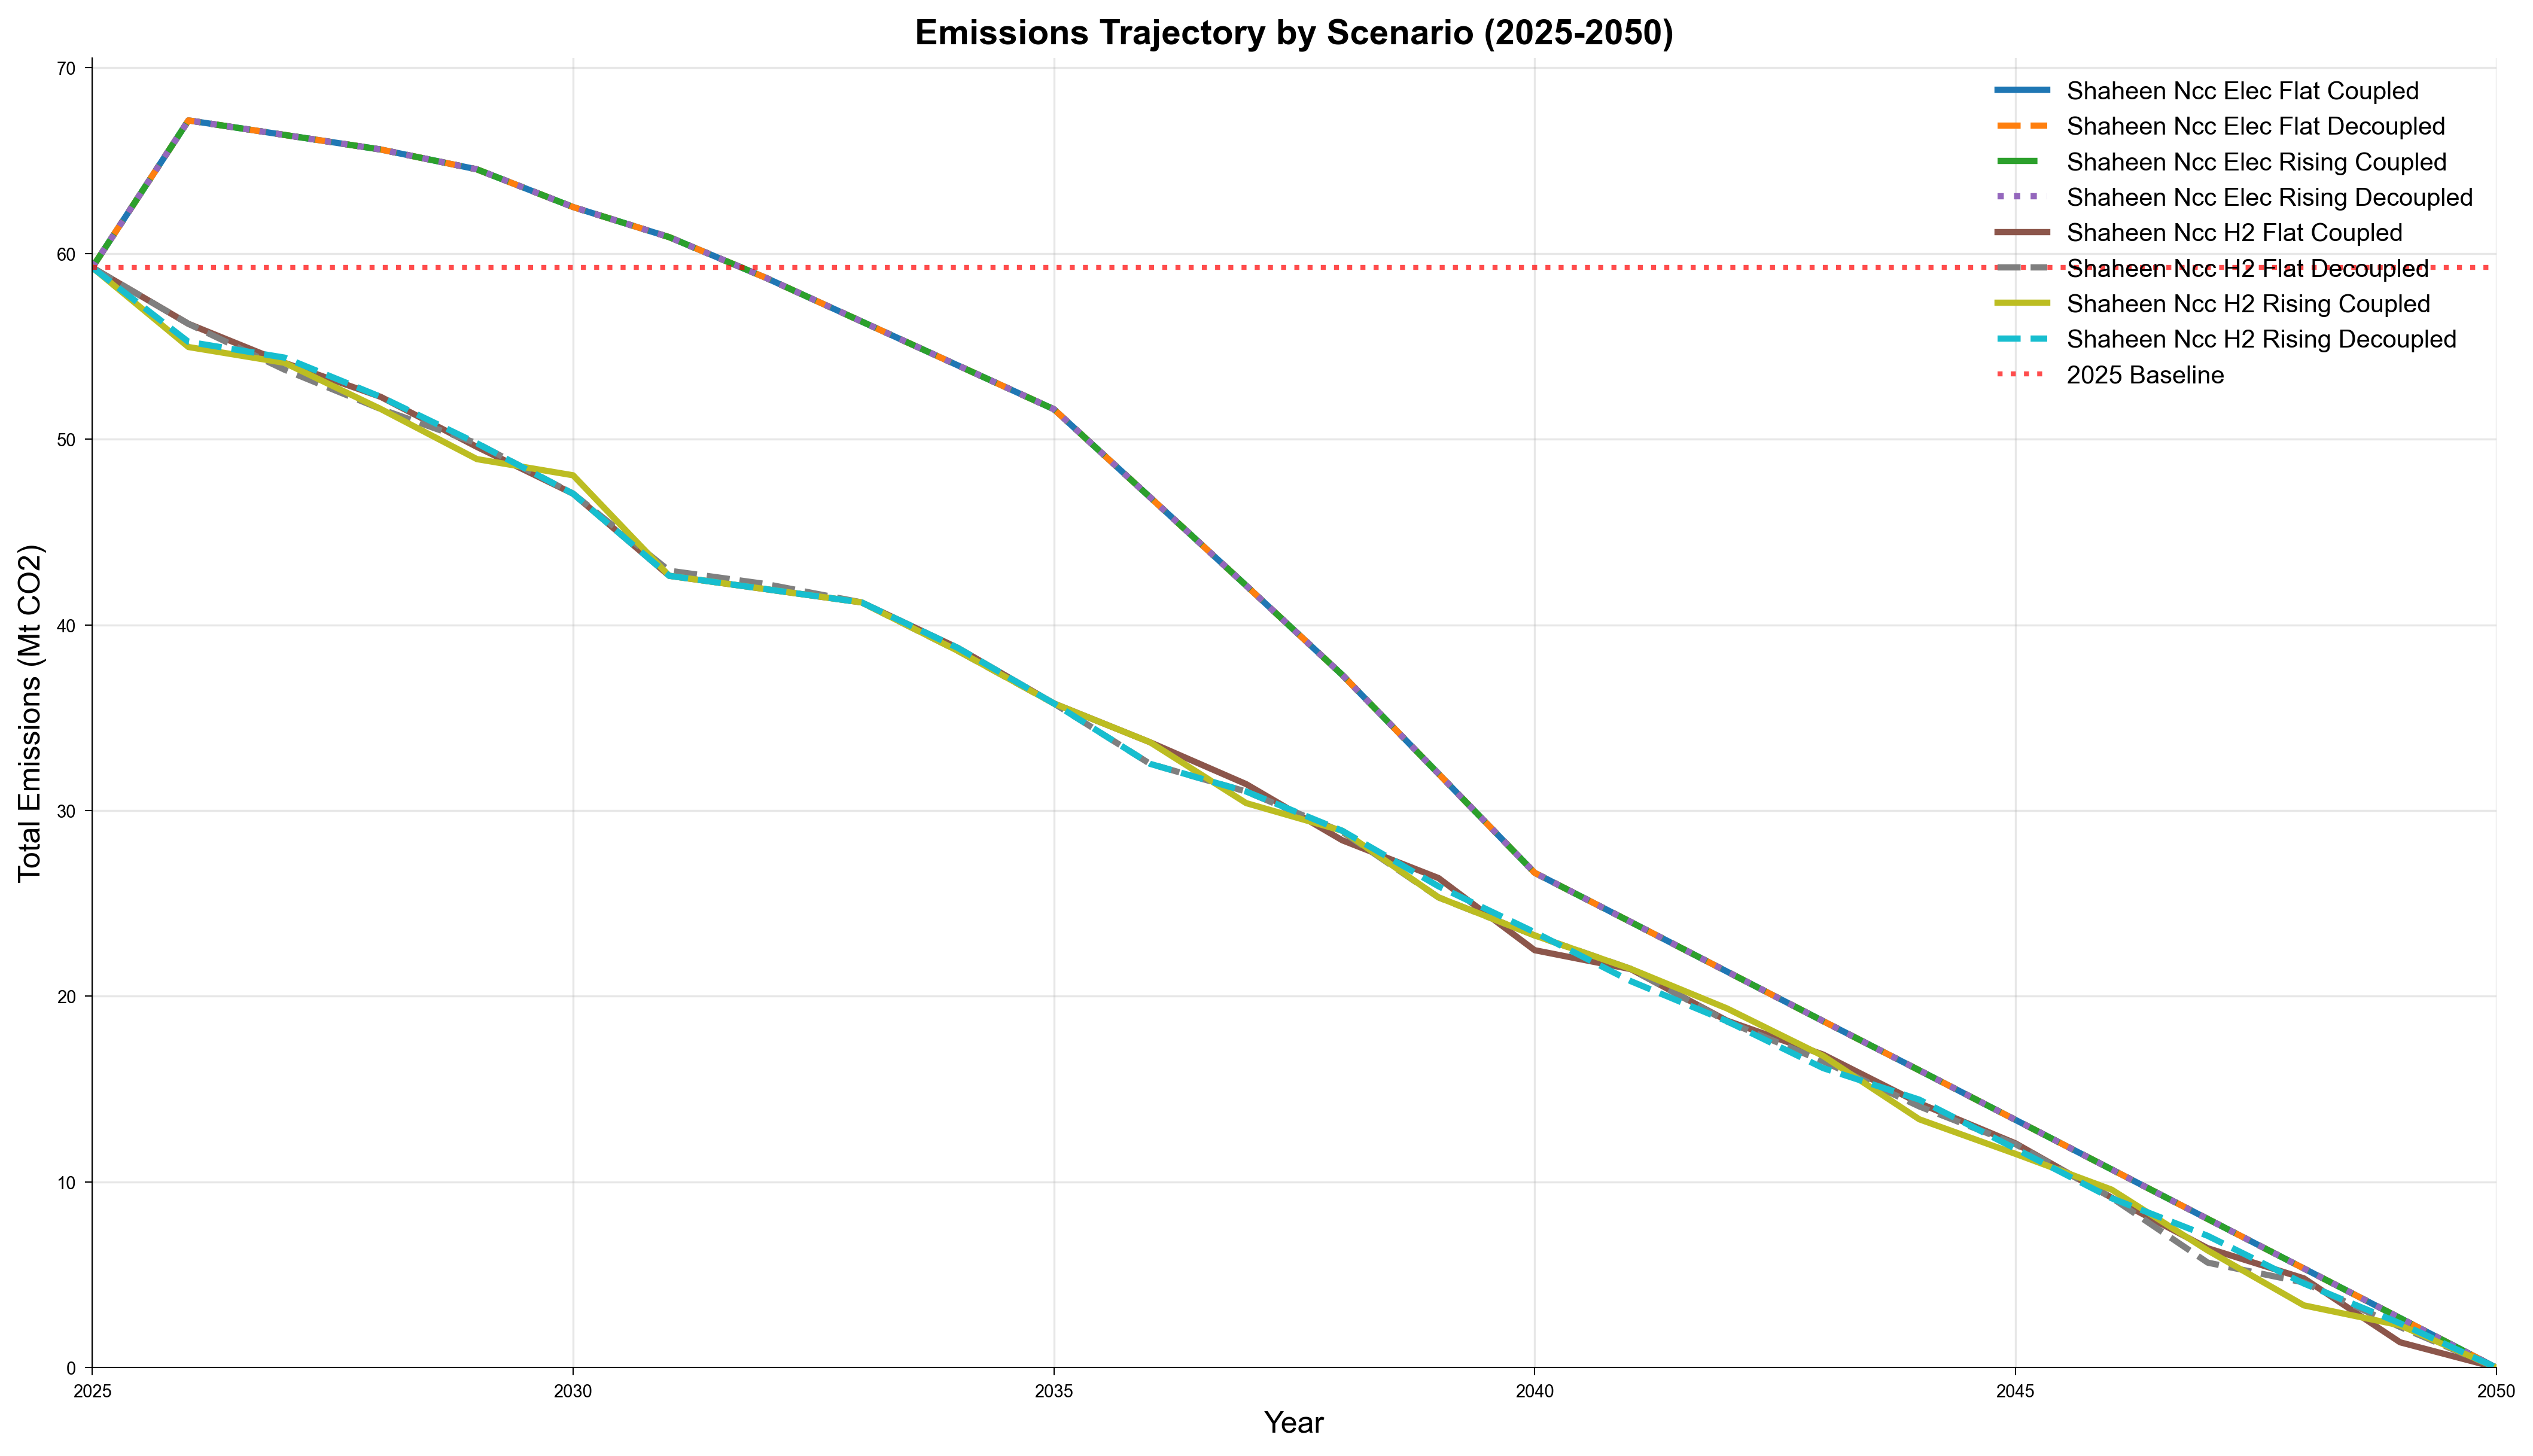
\includegraphics[width=0.95\textwidth]{../outputs/figures/report_emissions_trajectory.png}
\caption{Emissions trajectory by scenario (2025--2050). All scenarios achieve net-zero by 2050, but with varying reduction rates determined by production pathway and technology availability constraints.}
\label{fig:emissions_trajectory}
\end{figure}

Figure~\ref{fig:macc_curves} presents the marginal abatement cost curves for all six scenarios in 2050, illustrating the cost structure of achieving net-zero emissions.

\begin{figure}[H]
\centering
\includegraphics[width=0.98\textwidth]{../outputs/figures/report_macc_curves_v2.png}
\caption{Marginal Abatement Cost Curves for all six scenarios (2050). Step functions show cumulative abatement potential (Mt~\COtwo) versus marginal cost (\$/t~\COtwo). Horizontal dashed lines indicate carbon price reference levels (\$50, \$100, \$200/t~\COtwo). Summary statistics boxes show total abatement and weighted average MAC for each scenario. H2-based scenarios generally exhibit lower average MACs than electric alternatives.}
\label{fig:macc_curves}
\end{figure}

\subsection{Regional Analysis}

Emissions are concentrated in three major petrochemical complexes. Table~\ref{tab:regional_emissions} presents the regional distribution of baseline emissions.

\begin{table}[H]
\centering
\caption{Regional Baseline Emissions and Share}
\label{tab:regional_emissions}
\begin{tabular}{@{}lrrl@{}}
\toprule
\textbf{Region} & \textbf{Emissions} & \textbf{Share} & \textbf{Key Companies} \\
 & (Mt \COtwo) & (\%) & \\
\midrule
Yeosu & 22.41 & 37.8 & Yeochon NCC, Lotte Chemical, LG Chem \\
Daesan & 17.22 & 29.1 & Hanwha TotalEnergies, LG Chem \\
Ulsan & 14.81--19.24$^*$ & 25.0--32.5 & SK Geocentric, S-Oil, Daehan Oil \\
Other & 0.38 & 0.6 & Various \\
\bottomrule
\multicolumn{4}{l}{\footnotesize $^*$Ulsan emissions vary due to Shaheen project additions.}
\end{tabular}
\end{table}

Figure~\ref{fig:regional_heatmap} presents the evolution of regional emissions over time under the Shaheen NCC-H2 scenario.

\begin{figure}[H]
\centering
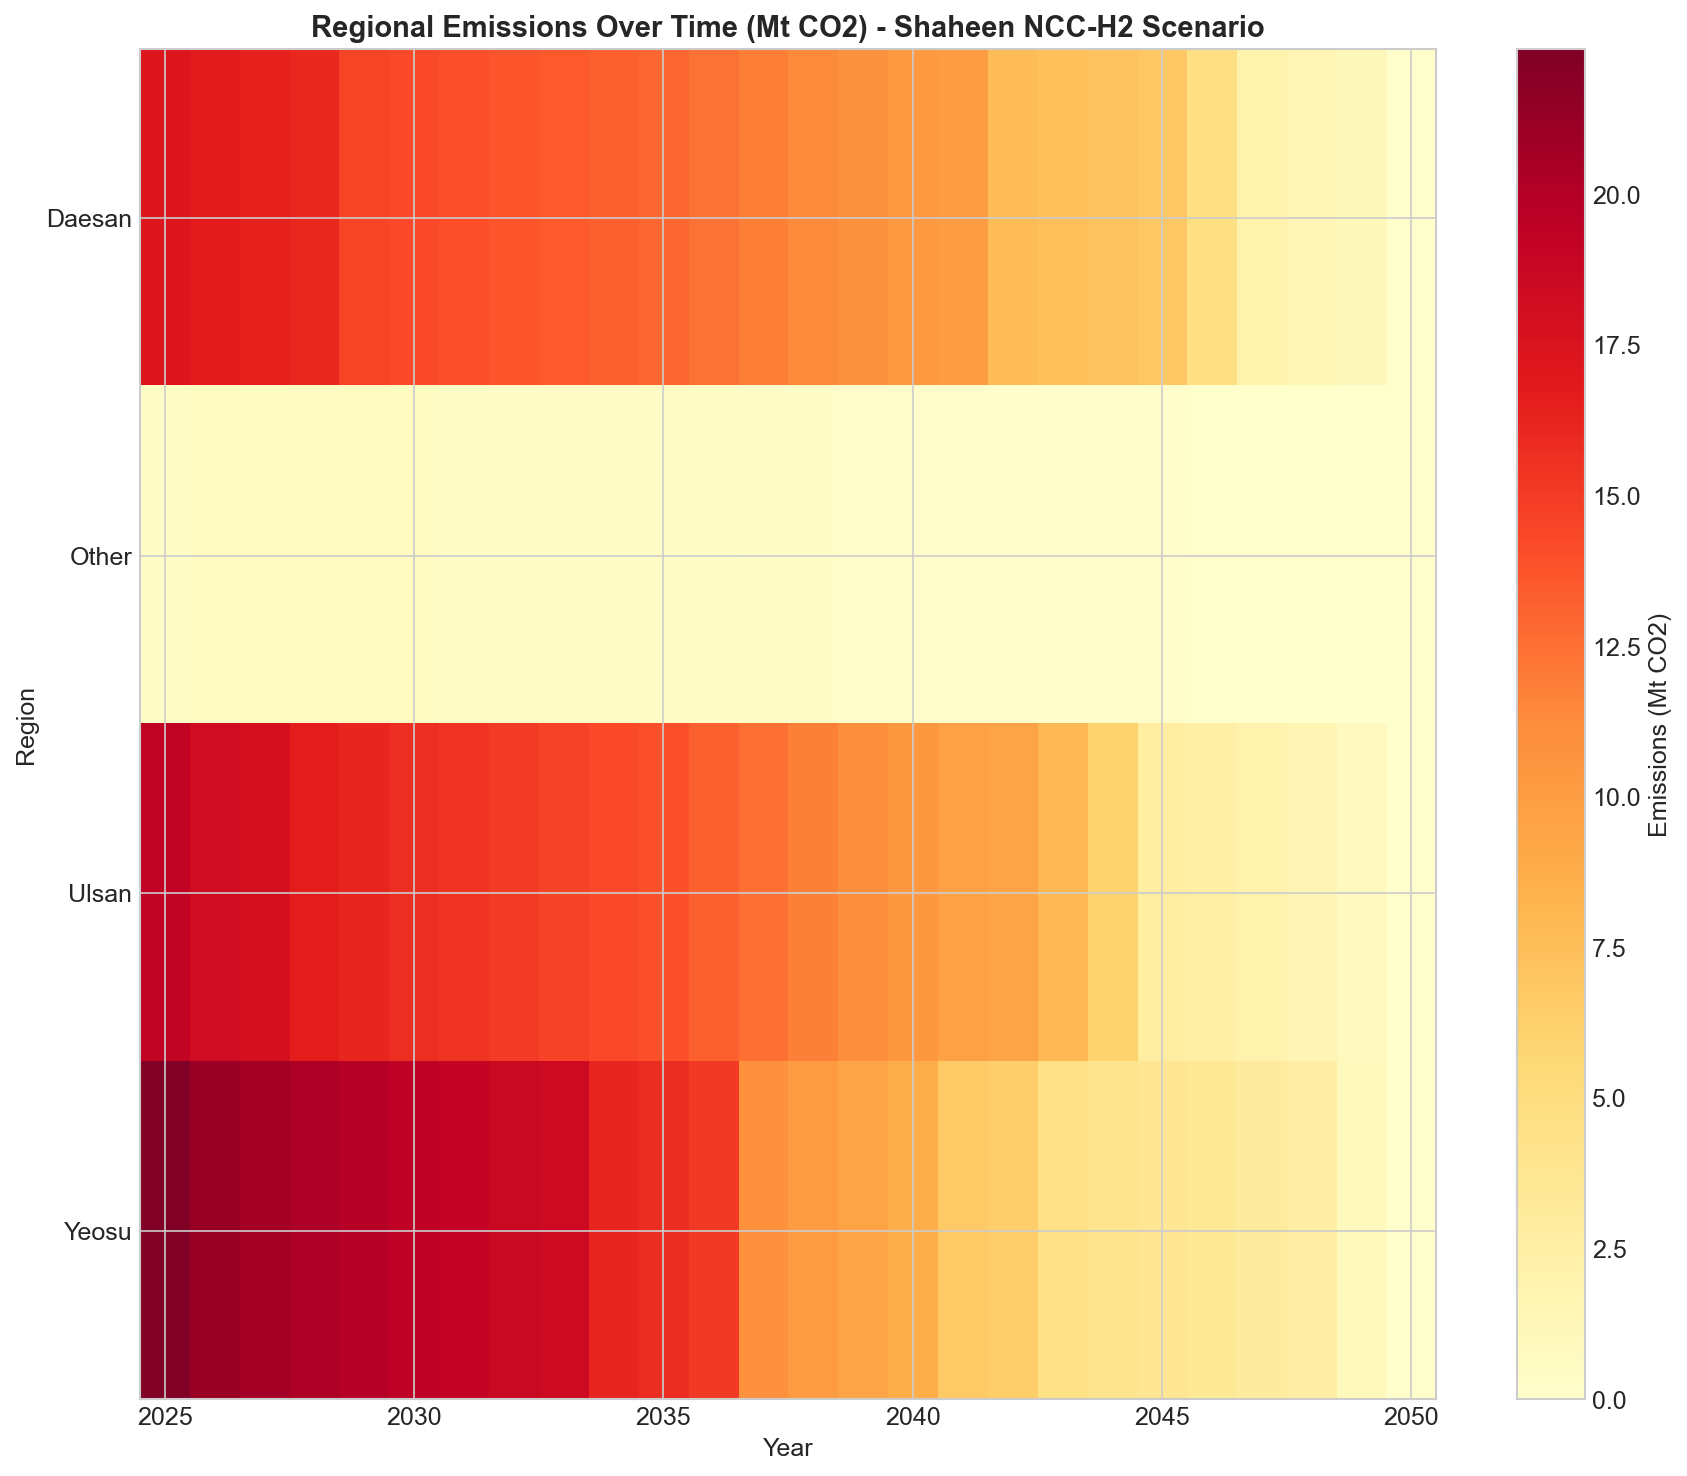
\includegraphics[width=0.85\textwidth]{../outputs/figures/report_regional_heatmap.png}
\caption{Regional emissions heatmap showing emissions intensity (Mt~\COtwo) by region and year under the Shaheen NCC-H2 scenario. Darker colors indicate higher emissions.}
\label{fig:regional_heatmap}
\end{figure}

\subsection{Company Analysis}

Emissions are highly concentrated among a small number of companies. Table~\ref{tab:company_emissions} presents the top ten emitters.

\begin{table}[H]
\centering
\caption{Top 10 Companies by Baseline Emissions}
\label{tab:company_emissions}
\begin{tabular}{@{}clrrl@{}}
\toprule
\textbf{Rank} & \textbf{Company} & \textbf{Emissions} & \textbf{Share} & \textbf{Primary Location} \\
 & & (Mt \COtwo) & (\%) & \\
\midrule
1 & LG Chem & 14.36 & 18.4 & Daesan, Yeosu \\
2 & Lotte Chemical & 11.20 & 14.3 & Daesan, Yeosu \\
3 & Yeochon NCC & 8.62 & 11.0 & Yeosu \\
4 & Hanwha TotalEnergies & 7.44 & 9.5 & Daesan \\
5 & GS Caltex & 5.19 & 6.6 & Yeosu \\
6 & SK Geocentric & 5.01 & 6.4 & Ulsan \\
7 & HD Hyundai Chemical & 4.96 & 6.3 & Daesan \\
8 & Daehan Oil Chemical & 3.86 & 4.9 & Ulsan \\
9 & S-Oil & 2.98 & 3.8 & Ulsan \\
10 & Hanwha Solutions & 2.01 & 2.6 & Yeosu, Ulsan \\
\midrule
 & \textbf{Top 10 Total} & \textbf{65.62} & \textbf{83.9} & \\
 & Other (51 companies) & 12.63 & 16.1 & Various \\
\bottomrule
\end{tabular}
\end{table}

The top four companies---LG Chem, Lotte Chemical, Yeochon NCC, and Hanwha TotalEnergies---account for 53.2\% of total industry emissions. These companies will bear the largest absolute transition costs and face the greatest stranded asset exposure under stringent carbon budget scenarios.

Figure~\ref{fig:top5_companies} presents a comprehensive analysis of the top five emitting companies, including baseline emissions, stranding risk exposure, company-level MACC curves, transition investment requirements, and technology deployment mix.

\begin{figure}[H]
\centering
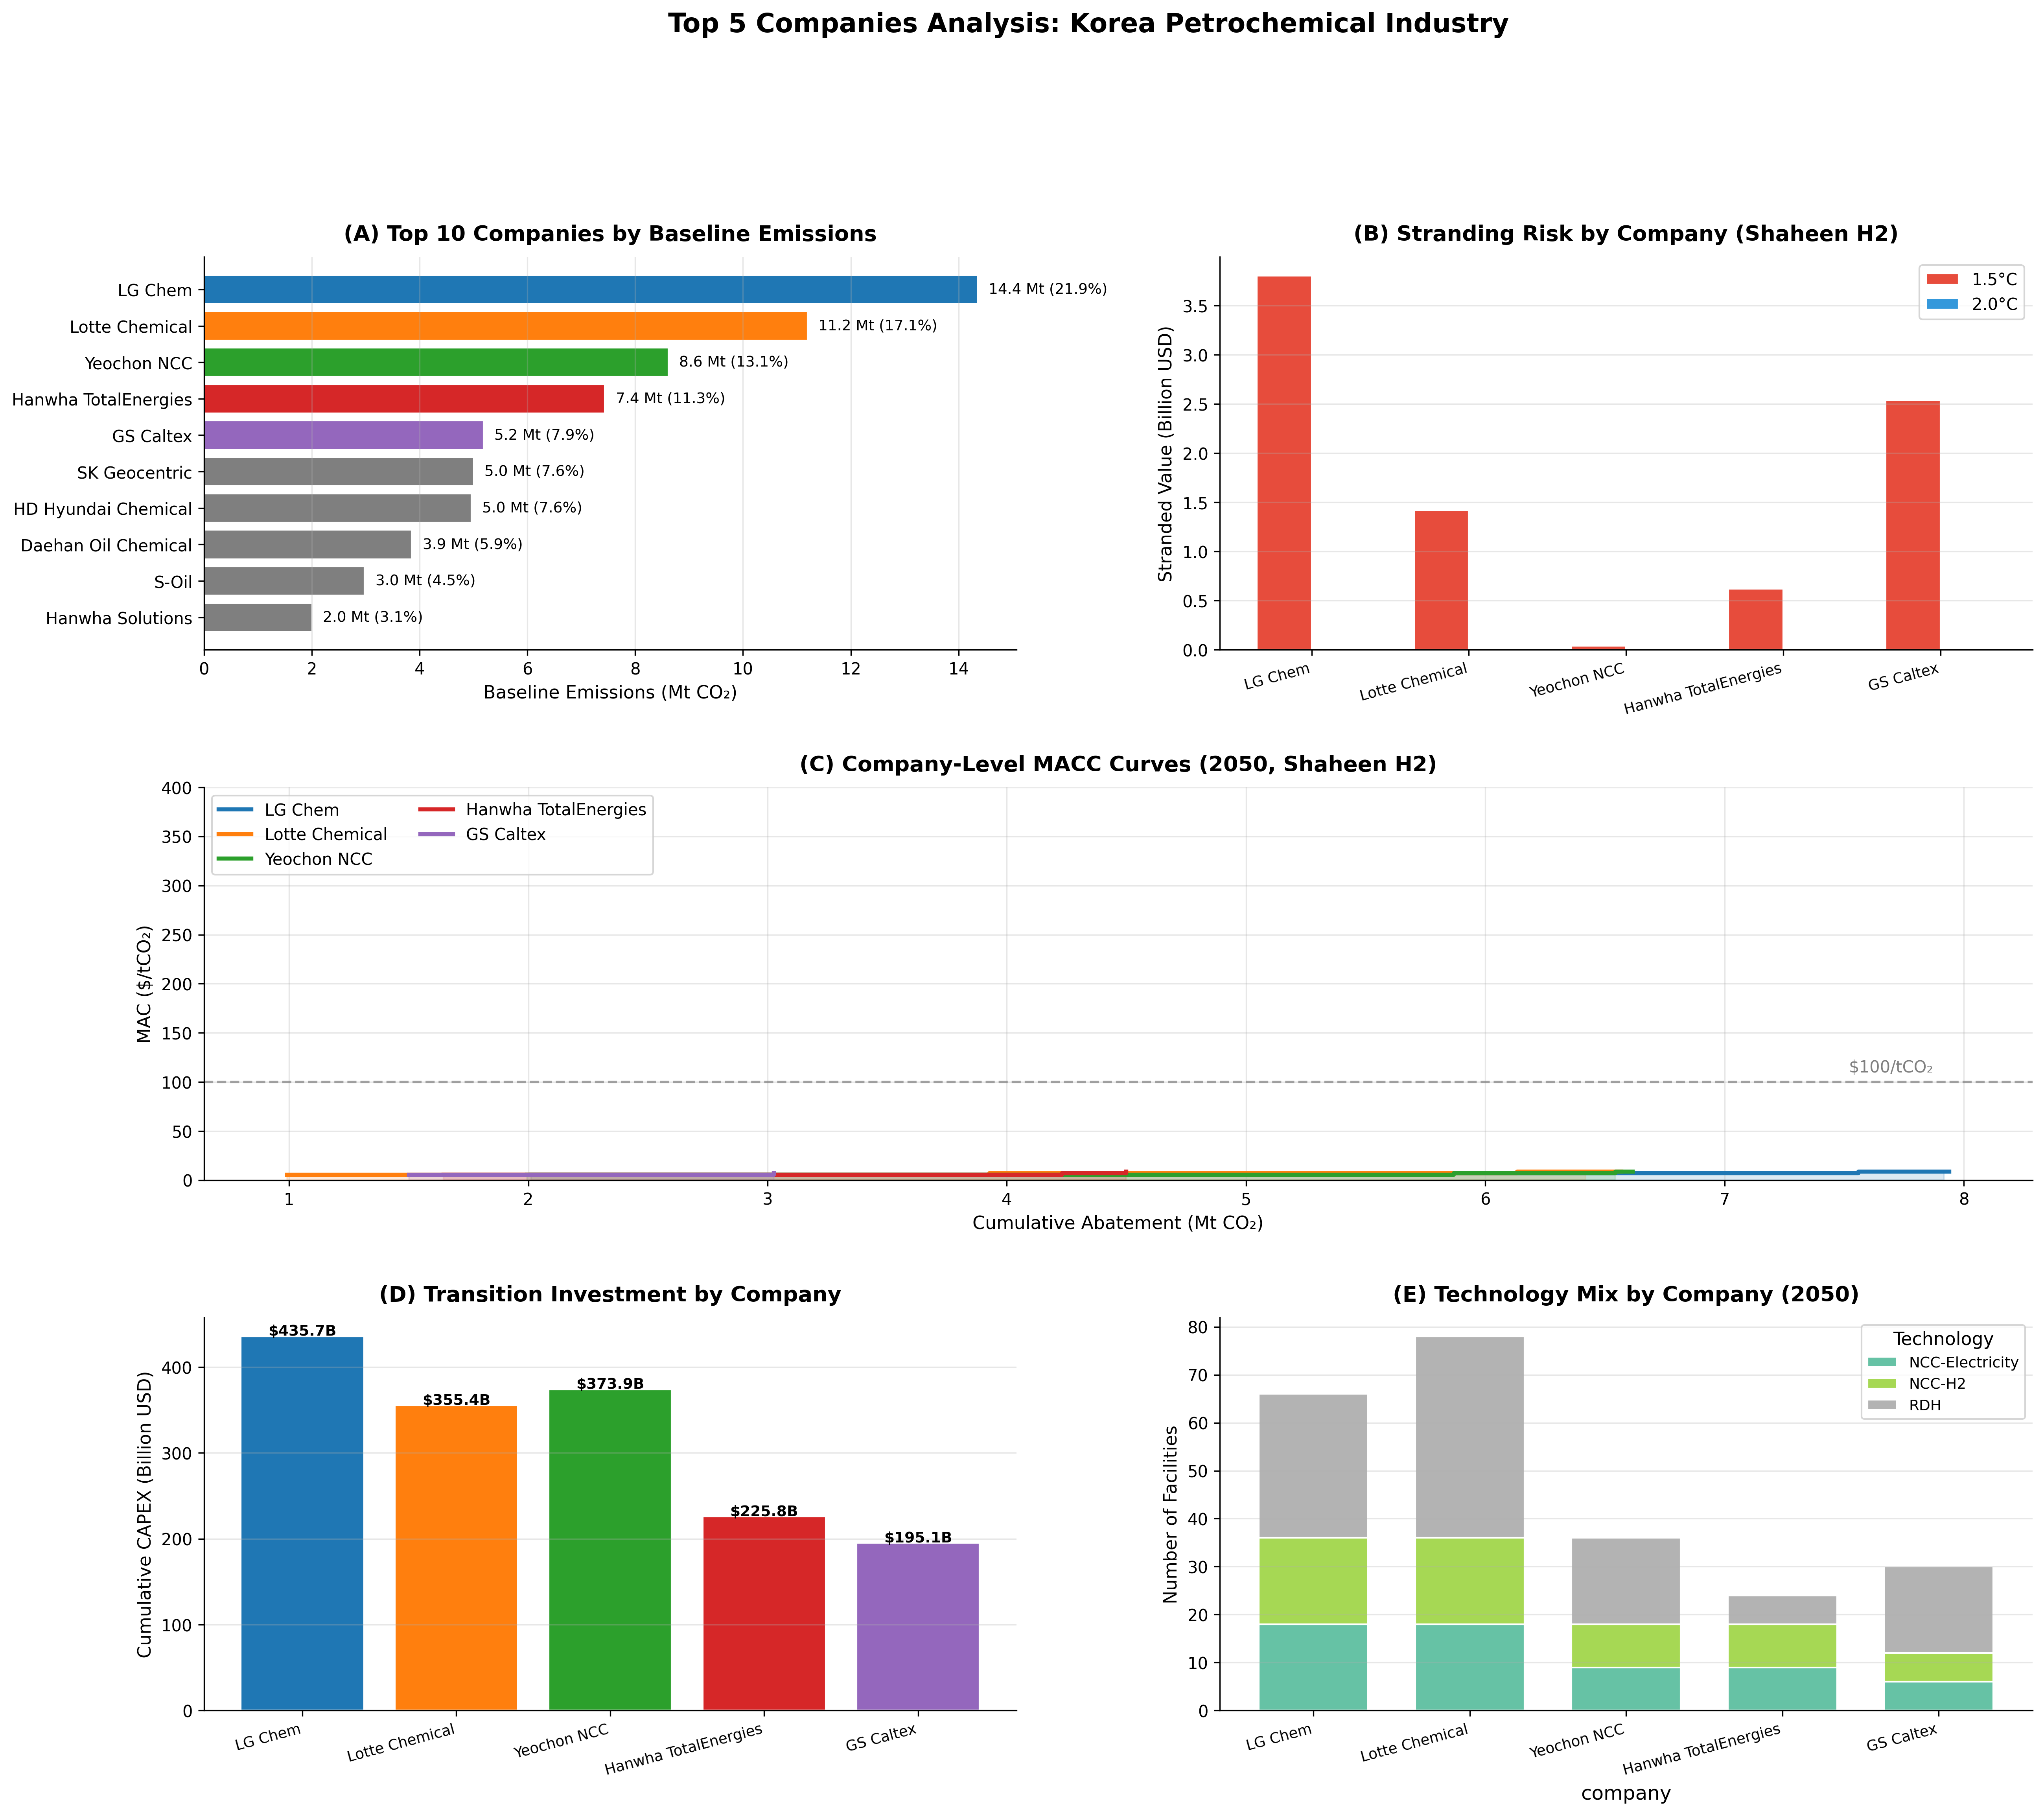
\includegraphics[width=0.98\textwidth]{../outputs/figures/report_top5_companies.png}
\caption{Top 5 companies analysis: (A) Baseline emissions showing LG Chem as the largest emitter at 14.4 Mt~\COtwo; (B) Stranding risk under 1.5°C vs. 2.0°C pathways; (C) Company-level MACC curves with \$100/t~\COtwo reference line; (D) Cumulative transition CAPEX requirements; (E) Technology deployment mix in 2050 by company. The top five companies account for 59.8\% of total sectoral emissions and face proportionally higher transition costs and stranded asset exposure.}
\label{fig:top5_companies}
\end{figure}

%%%%%%%%%%%%%%%%%%%%%%%%%%%%%%%%%%%%%%%%%%%%%%%%%%%%%%%%%%%%%%%%%%%%%%%%%%%%%%%
%% 5. Technology Analysis
%%%%%%%%%%%%%%%%%%%%%%%%%%%%%%%%%%%%%%%%%%%%%%%%%%%%%%%%%%%%%%%%%%%%%%%%%%%%%%%
\section{Technology Analysis}

\subsection{Technology Parameters}

Table~\ref{tab:tech_params} presents the key parameters for decarbonization technologies evaluated in this analysis.

\begin{table}[H]
\centering
\caption{Technology Parameters and Cost Trajectories}
\label{tab:tech_params}
\begin{tabular}{@{}llrrrrr@{}}
\toprule
\textbf{Technology} & \textbf{Application} & \textbf{TRL} & \textbf{Avail.} & \textbf{CAPEX '25} & \textbf{CAPEX '50} & \textbf{Life} \\
 & & & & (\$/t\COtwo) & (\$/t\COtwo) & (yr) \\
\midrule
Heat Pump & $<$165°C heat & 9 & 2025 & 800 & 400 & 20 \\
NCC-H2 & Naphtha crackers & 7 & 2030 & 1,700 & 850 & 25 \\
NCC-Electricity & Naphtha crackers & 8 & 2030 & 1,500 & 750 & 25 \\
RDH & BTX plants & 8 & 2026 & 900 & 450 & 25 \\
RE-PPA & Grid electricity & N/A & 2025 & 0 & 0 & 99 \\
\bottomrule
\end{tabular}
\end{table}

Technology readiness levels (TRL) and availability years are based on industry announcements and expert assessments. The BASF/SABIC/Linde electric cracker demonstration (TRL 8) informs the NCC-Electricity parameters \citep{basf2024}, while NCC-H2 reflects the lower maturity of hydrogen combustion systems for industrial-scale steam cracking \citep{iea2023hydrogen}.

\subsection{H2 vs. Electricity Pathway Comparison}

Figure~\ref{fig:h2_vs_elec} presents a comparative analysis of hydrogen-based and electric pathways across key metrics.

\begin{figure}[H]
\centering
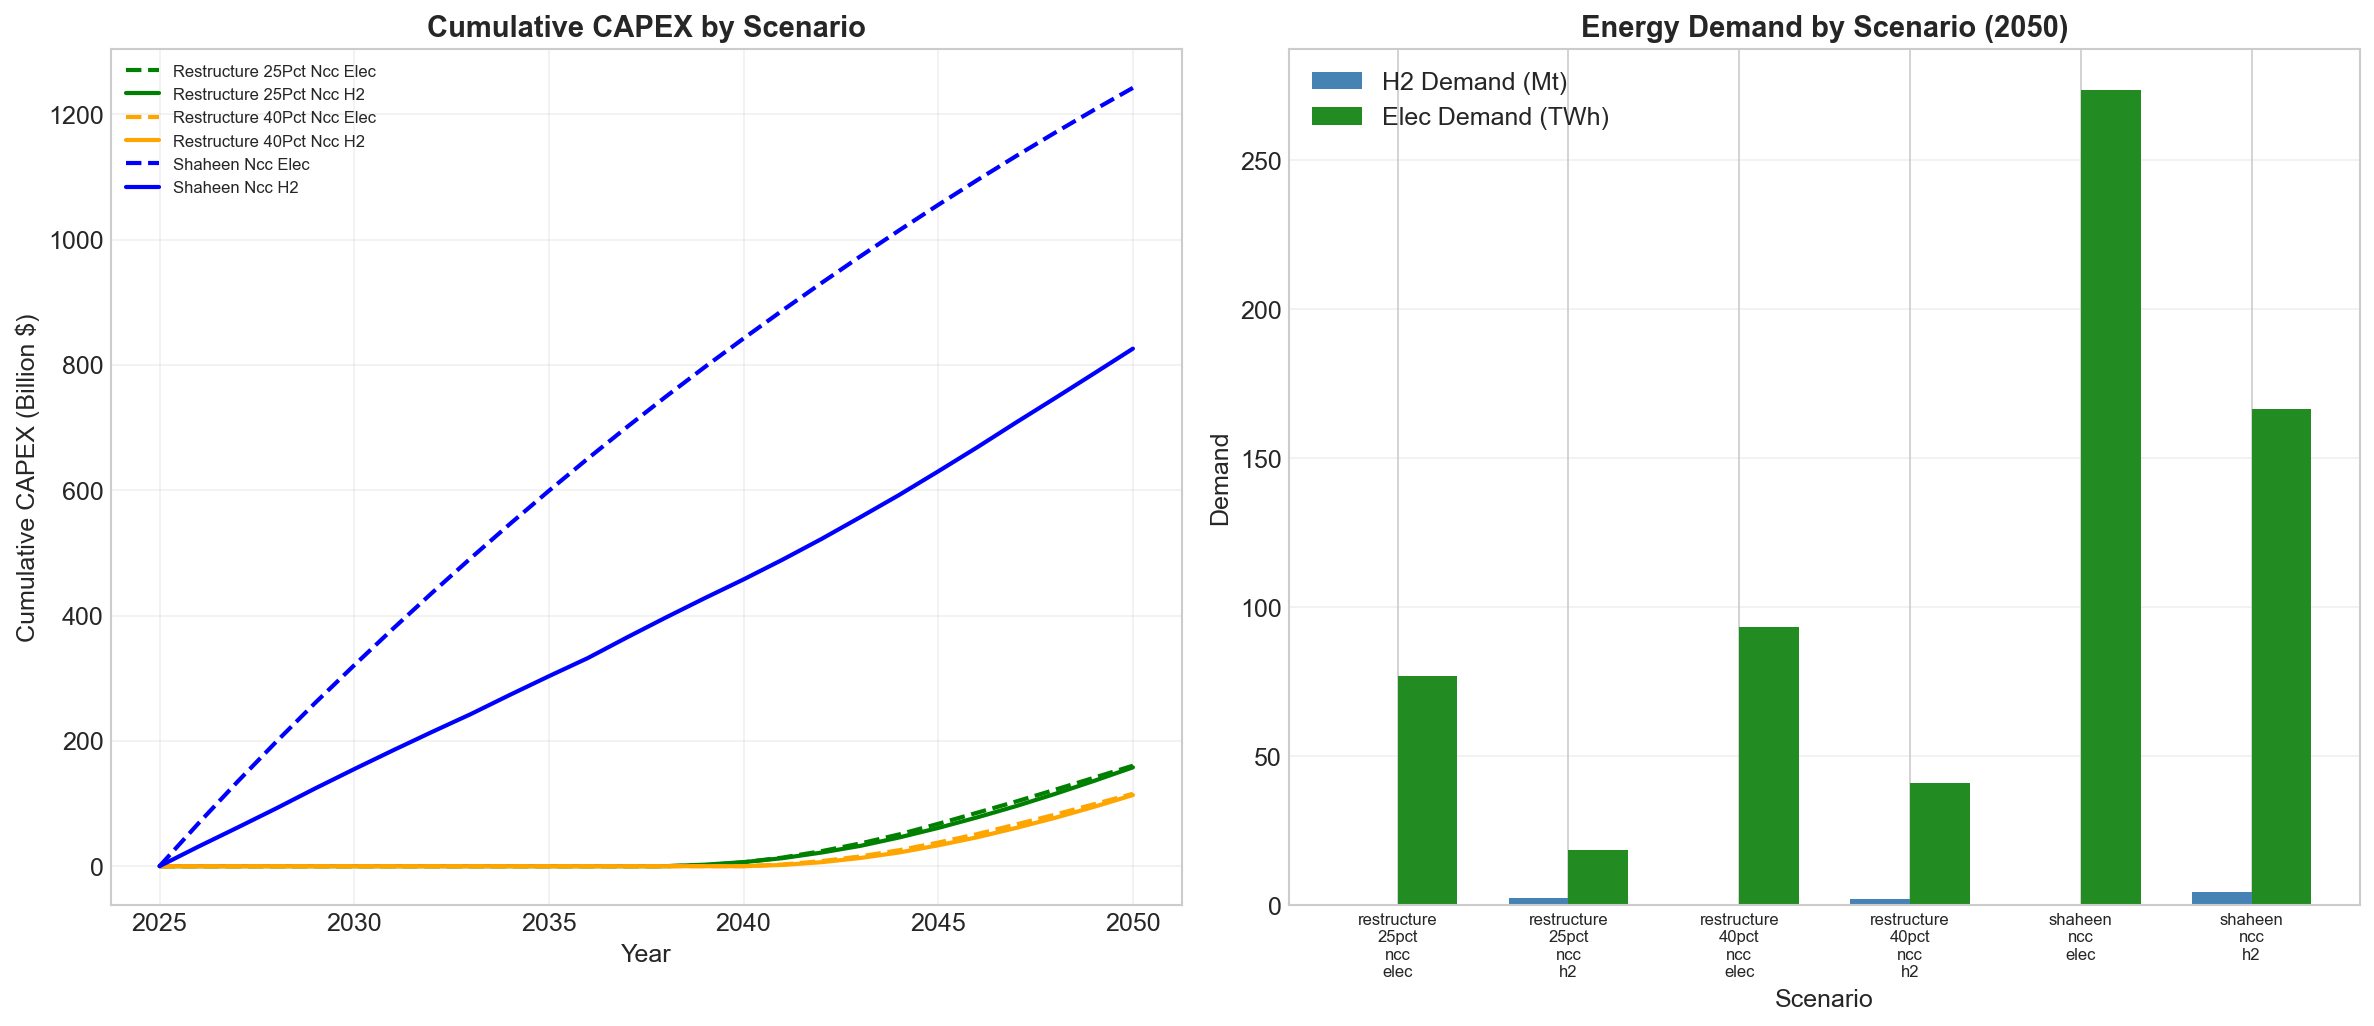
\includegraphics[width=0.95\textwidth]{../outputs/figures/report_h2_vs_elec.png}
\caption{Comparison of H2-based and electric pathways: (Left) Cumulative CAPEX trajectories; (Right) Final-year energy demands by scenario.}
\label{fig:h2_vs_elec}
\end{figure}

Key observations from the H2 vs. electricity comparison:

\begin{itemize}
\item \textbf{CAPEX:} H2-based scenarios show 28\% lower average cumulative CAPEX (\$365.7B vs. \$505.9B).
\item \textbf{Electricity Demand:} Electric scenarios require 96\% higher electricity demand on average (147.9 TWh vs. 75.3 TWh).
\item \textbf{Infrastructure:} H2 scenarios require substantial hydrogen infrastructure (2.0--4.3 Mt/year), while electric scenarios require expanded grid and RE-PPA capacity.
\item \textbf{Operating Costs:} Electric scenarios may achieve negative net operating costs due to fuel savings exceeding new electricity costs.
\end{itemize}

\subsection{Technology Deployment Timeline}

Figure~\ref{fig:tech_timeline} presents the technology deployment timeline under the Shaheen NCC-H2 scenario.

\begin{figure}[H]
\centering
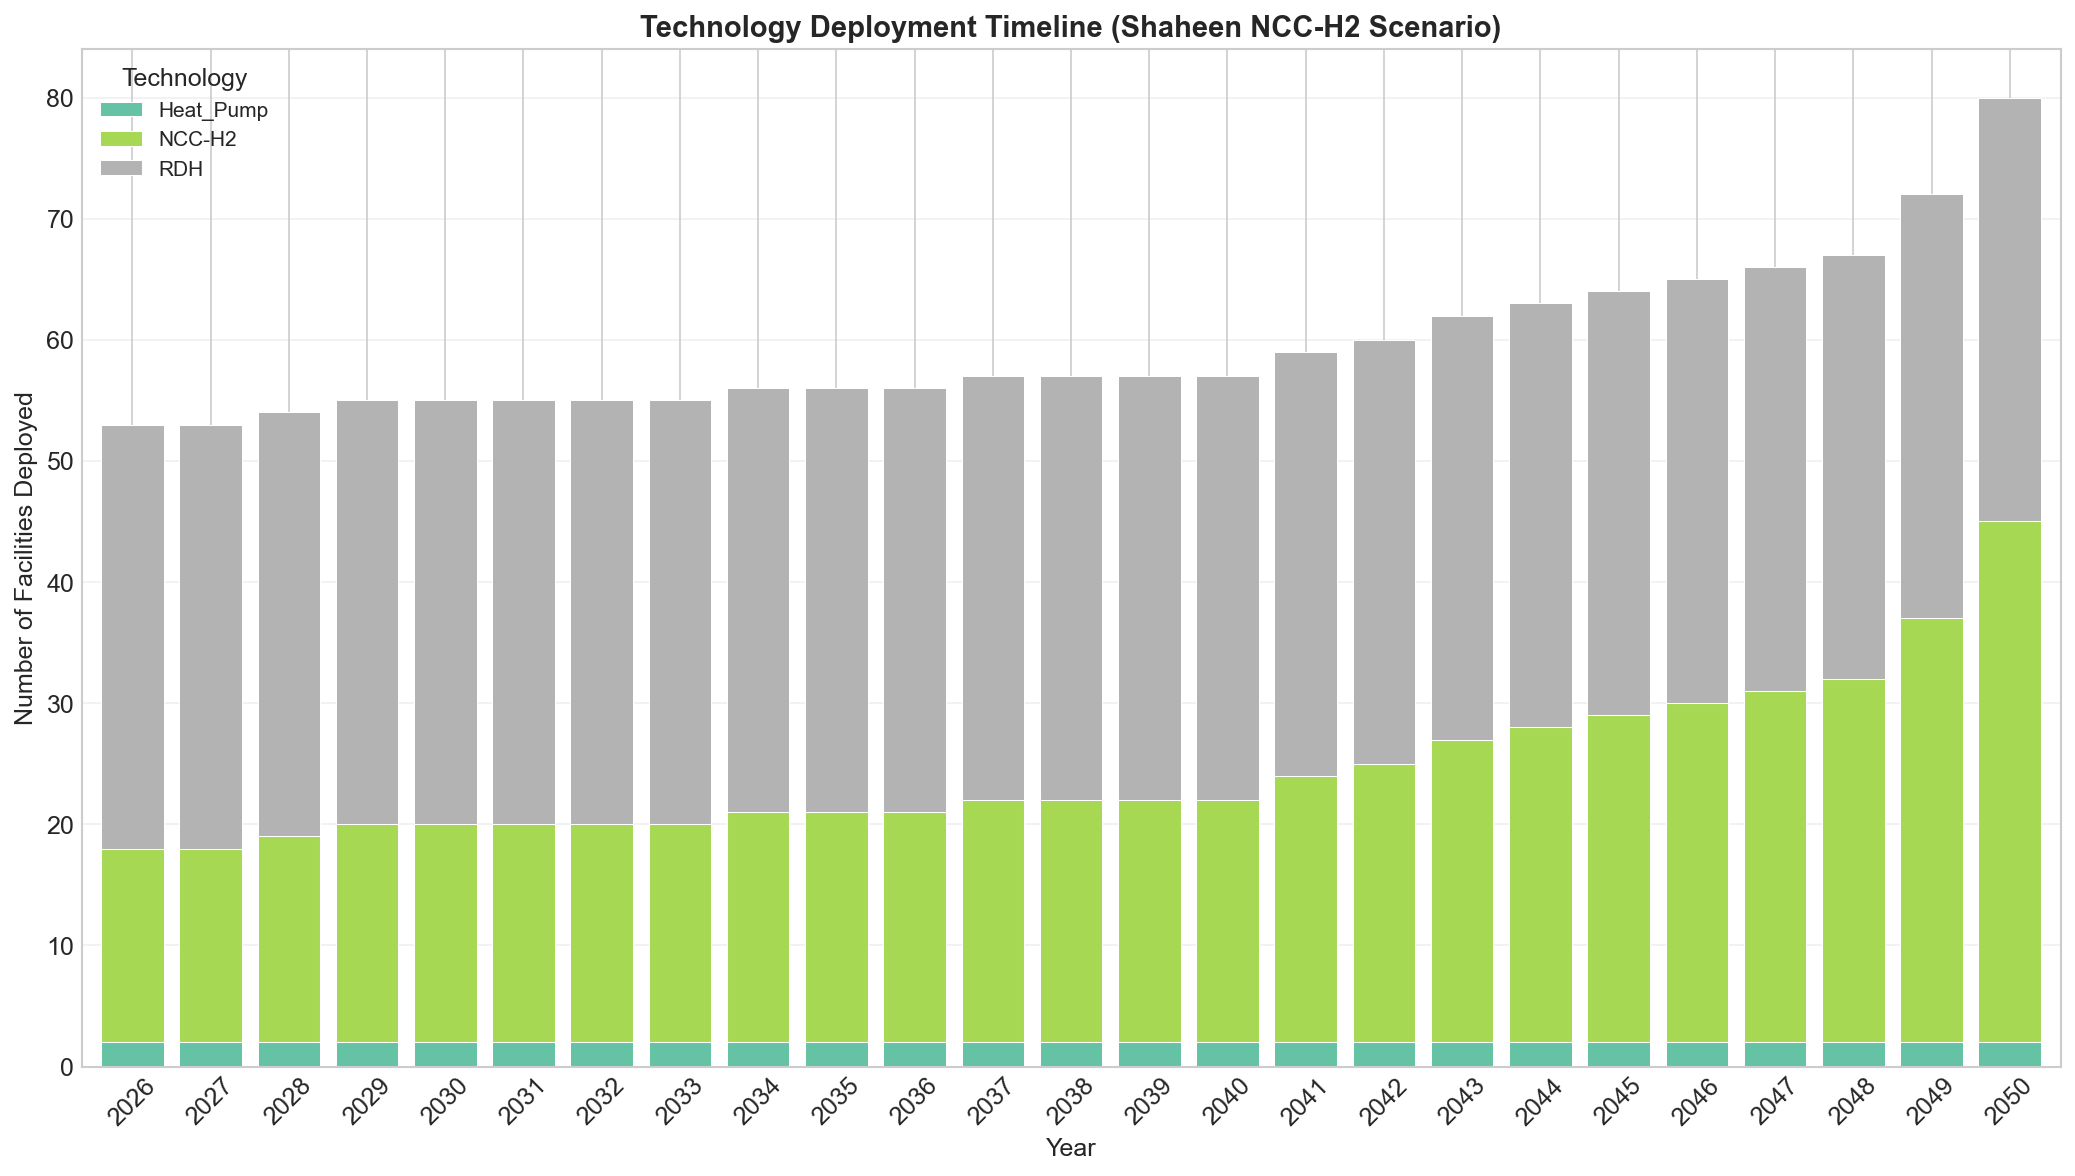
\includegraphics[width=0.95\textwidth]{../outputs/figures/report_tech_timeline.png}
\caption{Technology deployment timeline showing facility adoption by year under the Shaheen NCC-H2 scenario. Heat pumps deploy earliest (2025+), followed by RDH (2026+) and NCC-H2 (2030+).}
\label{fig:tech_timeline}
\end{figure}

The deployment pattern shows three distinct phases:
\begin{enumerate}
\item \textbf{Early Phase (2025--2029):} Heat pump deployment for low-temperature processes.
\item \textbf{Transition Phase (2030--2040):} RDH deployment for BTX plants and initial NCC technology deployment.
\item \textbf{Scale-up Phase (2040--2050):} Accelerated NCC technology deployment to achieve net-zero.
\end{enumerate}

%%%%%%%%%%%%%%%%%%%%%%%%%%%%%%%%%%%%%%%%%%%%%%%%%%%%%%%%%%%%%%%%%%%%%%%%%%%%%%%
%% 6. Financial Risk Analysis
%%%%%%%%%%%%%%%%%%%%%%%%%%%%%%%%%%%%%%%%%%%%%%%%%%%%%%%%%%%%%%%%%%%%%%%%%%%%%%%
\section{Financial Risk Analysis}

\subsection{Stranded Assets}

Table~\ref{tab:stranded_assets} presents the stranded asset exposure under different carbon budget pathways.

\begin{table}[H]
\centering
\caption{Stranded Asset Analysis by Scenario and Carbon Budget}
\label{tab:stranded_assets}
\begin{tabular}{@{}lrrrr@{}}
\toprule
\textbf{Scenario} & \textbf{1.5°C Year} & \textbf{1.5°C Value} & \textbf{2.0°C Year} & \textbf{2.0°C Value} \\
 & & (\$B) & & (\$B) \\
\midrule
shaheen\_ncc\_h2 & 2029 & 22.98 & 2050 & 5.27 \\
shaheen\_ncc\_elec & 2028 & 24.61 & 2042 & 10.43 \\
restructure\_25pct\_ncc\_h2 & 2032 & 14.41 & 2050 & 3.45 \\
restructure\_25pct\_ncc\_elec & 2032 & 14.41 & 2050 & 3.45 \\
restructure\_40pct\_ncc\_h2 & 2030 & 16.75 & 2050 & 3.45 \\
restructure\_40pct\_ncc\_elec & 2030 & 16.75 & 2050 & 3.45 \\
\bottomrule
\end{tabular}
\end{table}

Figure~\ref{fig:stranded_assets} presents a comprehensive four-panel analysis of stranded asset risk across scenarios and climate pathways.

\begin{figure}[H]
\centering
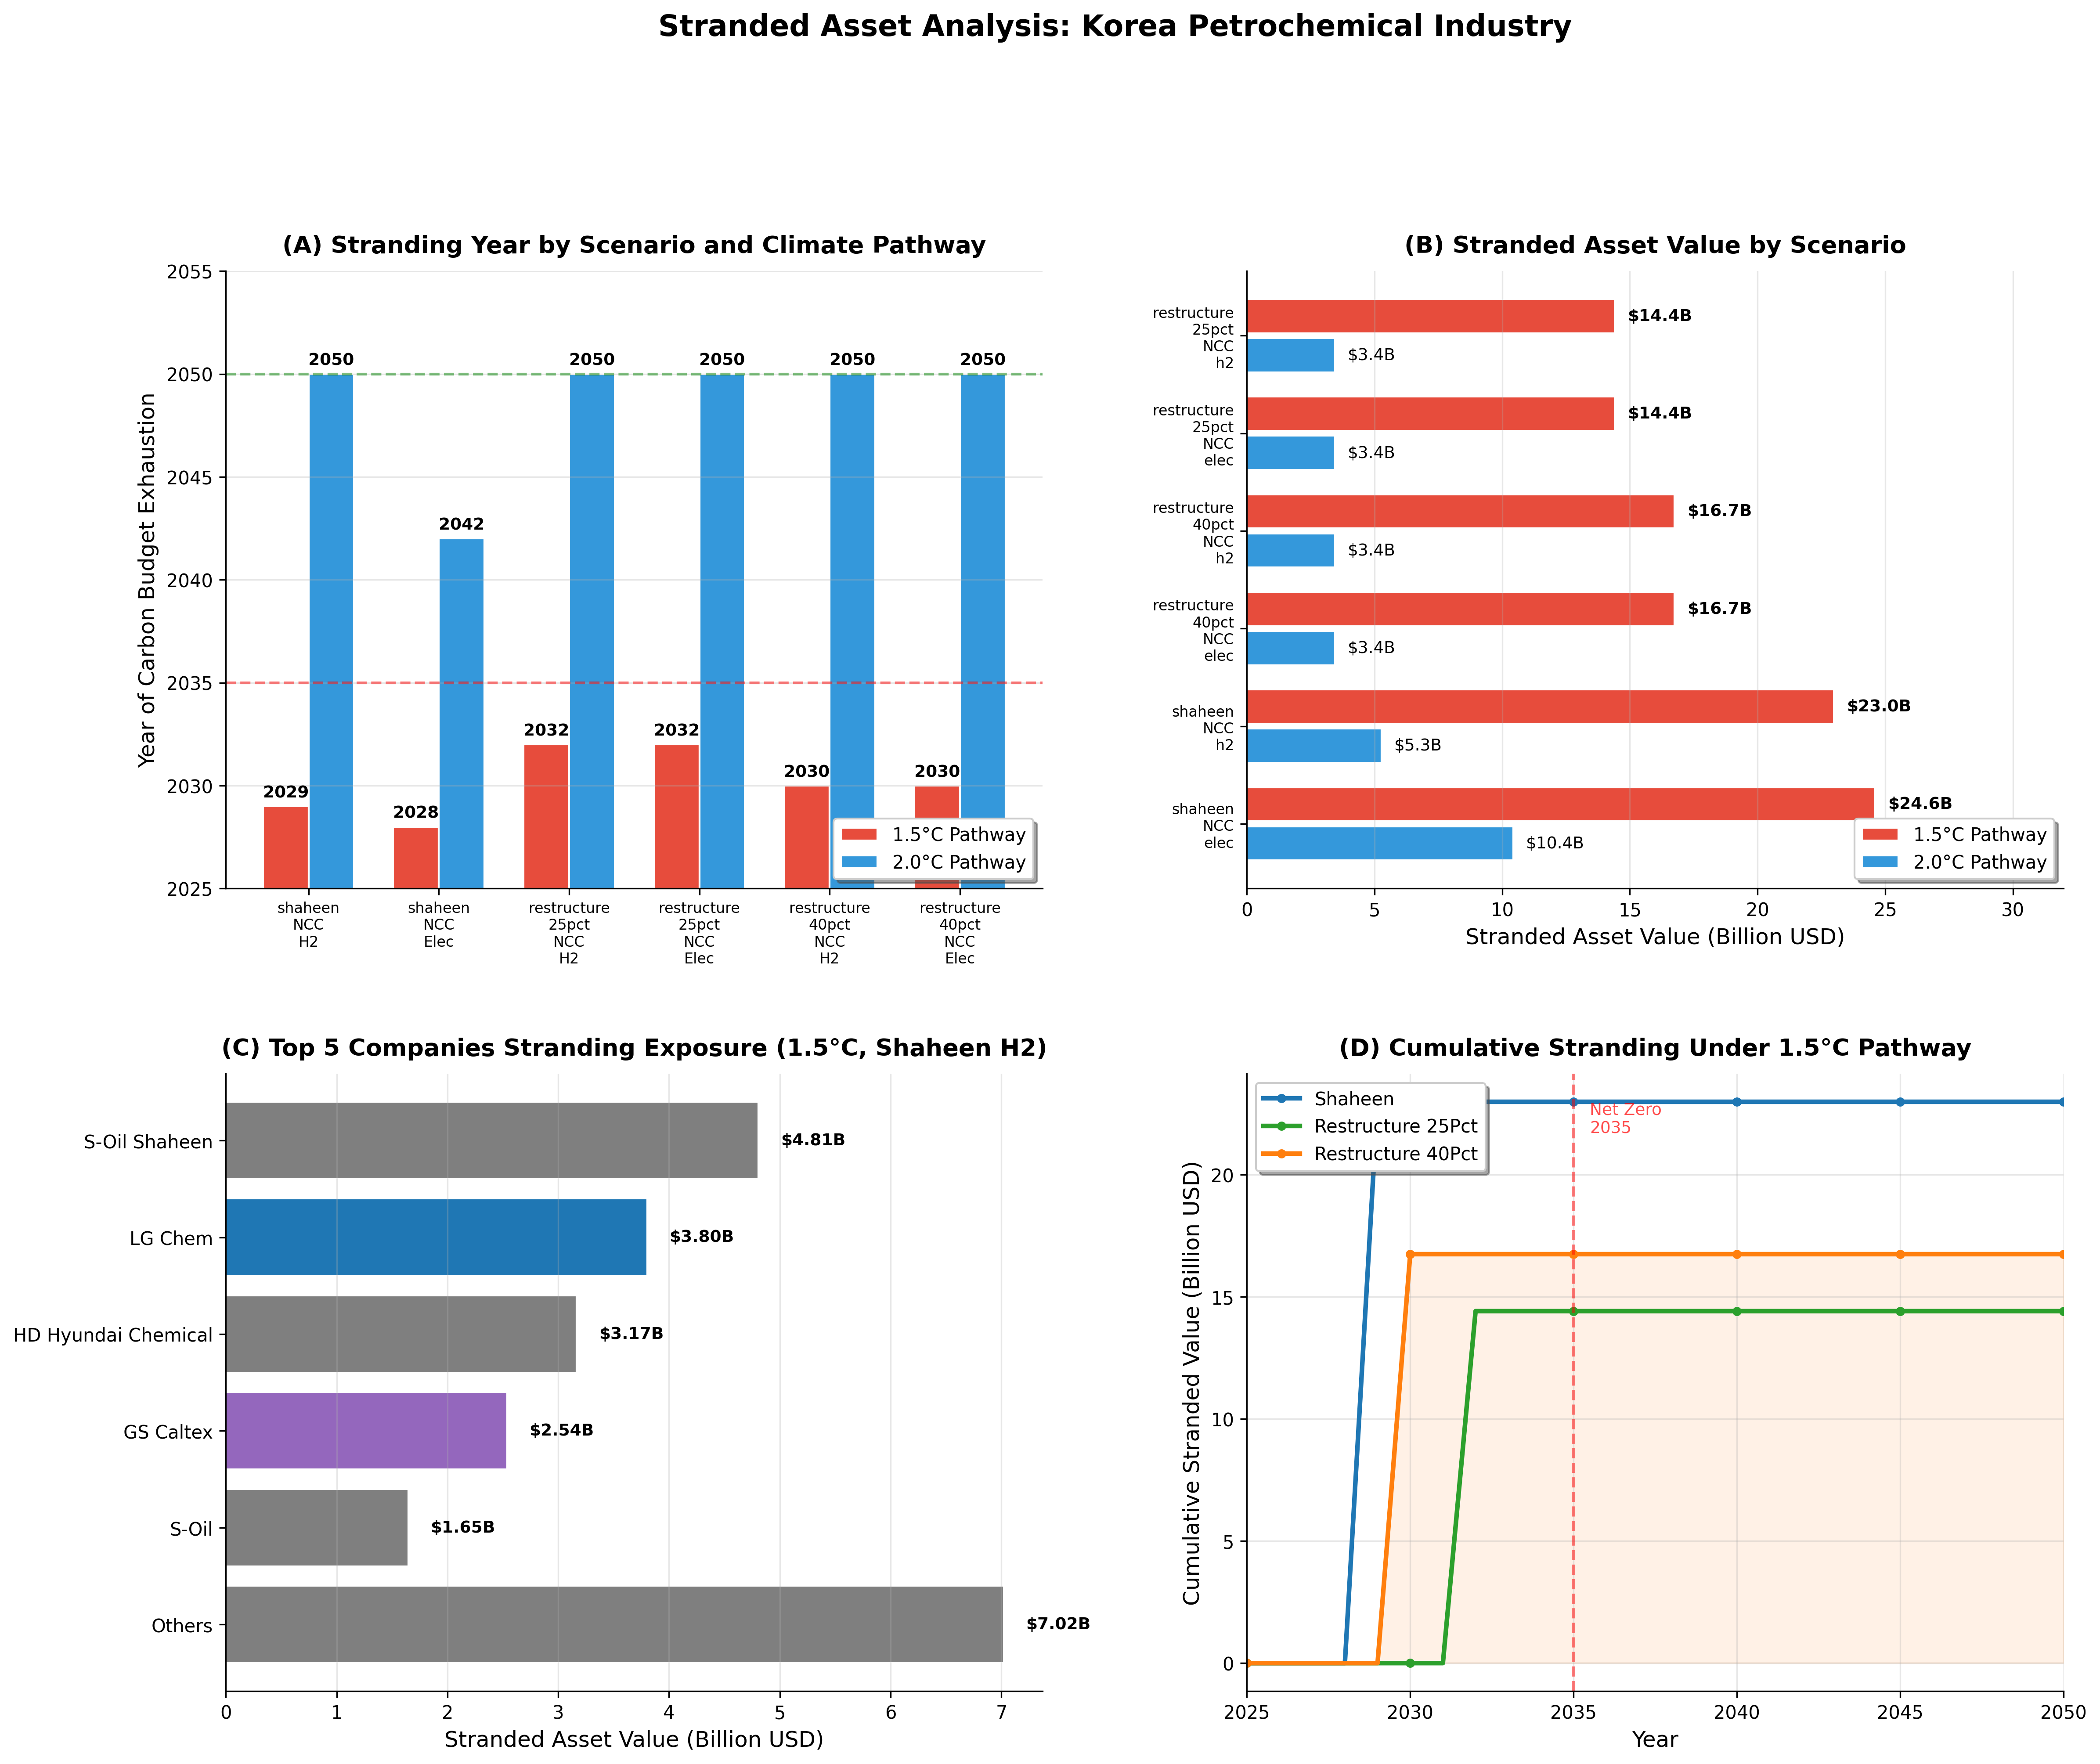
\includegraphics[width=0.98\textwidth]{../outputs/figures/report_stranded_assets_v2.png}
\caption{Stranded asset analysis: (A) Year of carbon budget exhaustion by scenario and climate pathway, showing earlier stranding under 1.5°C; (B) Stranded asset values in billion USD, sorted by risk exposure; (C) Top 5 companies' stranding exposure under the 1.5°C Shaheen H2 scenario; (D) Cumulative stranding trajectory over 2025--2050 for H2 scenarios under 1.5°C pathway. Red dashed lines indicate key policy milestones (2035 net-zero, 2050 target).}
\label{fig:stranded_assets}
\end{figure}

Key findings on stranded assets:
\begin{itemize}
\item The 1.5°C pathway creates \$14.4B--\$24.6B in stranded assets across all scenarios.
\item Electric scenarios face earlier stranding years (2028 vs. 2029--2032 for H2).
\item Restructuring reduces stranded asset exposure by 30--40\% compared to growth scenarios.
\item The 2.0°C pathway substantially reduces stranding risk (\$3.45B--\$10.43B).
\end{itemize}

\subsection{Facility-Level Cost Distribution}

Figure~\ref{fig:facility_scatter} presents the facility-level distribution of marginal abatement costs and abatement potential.

\begin{figure}[H]
\centering
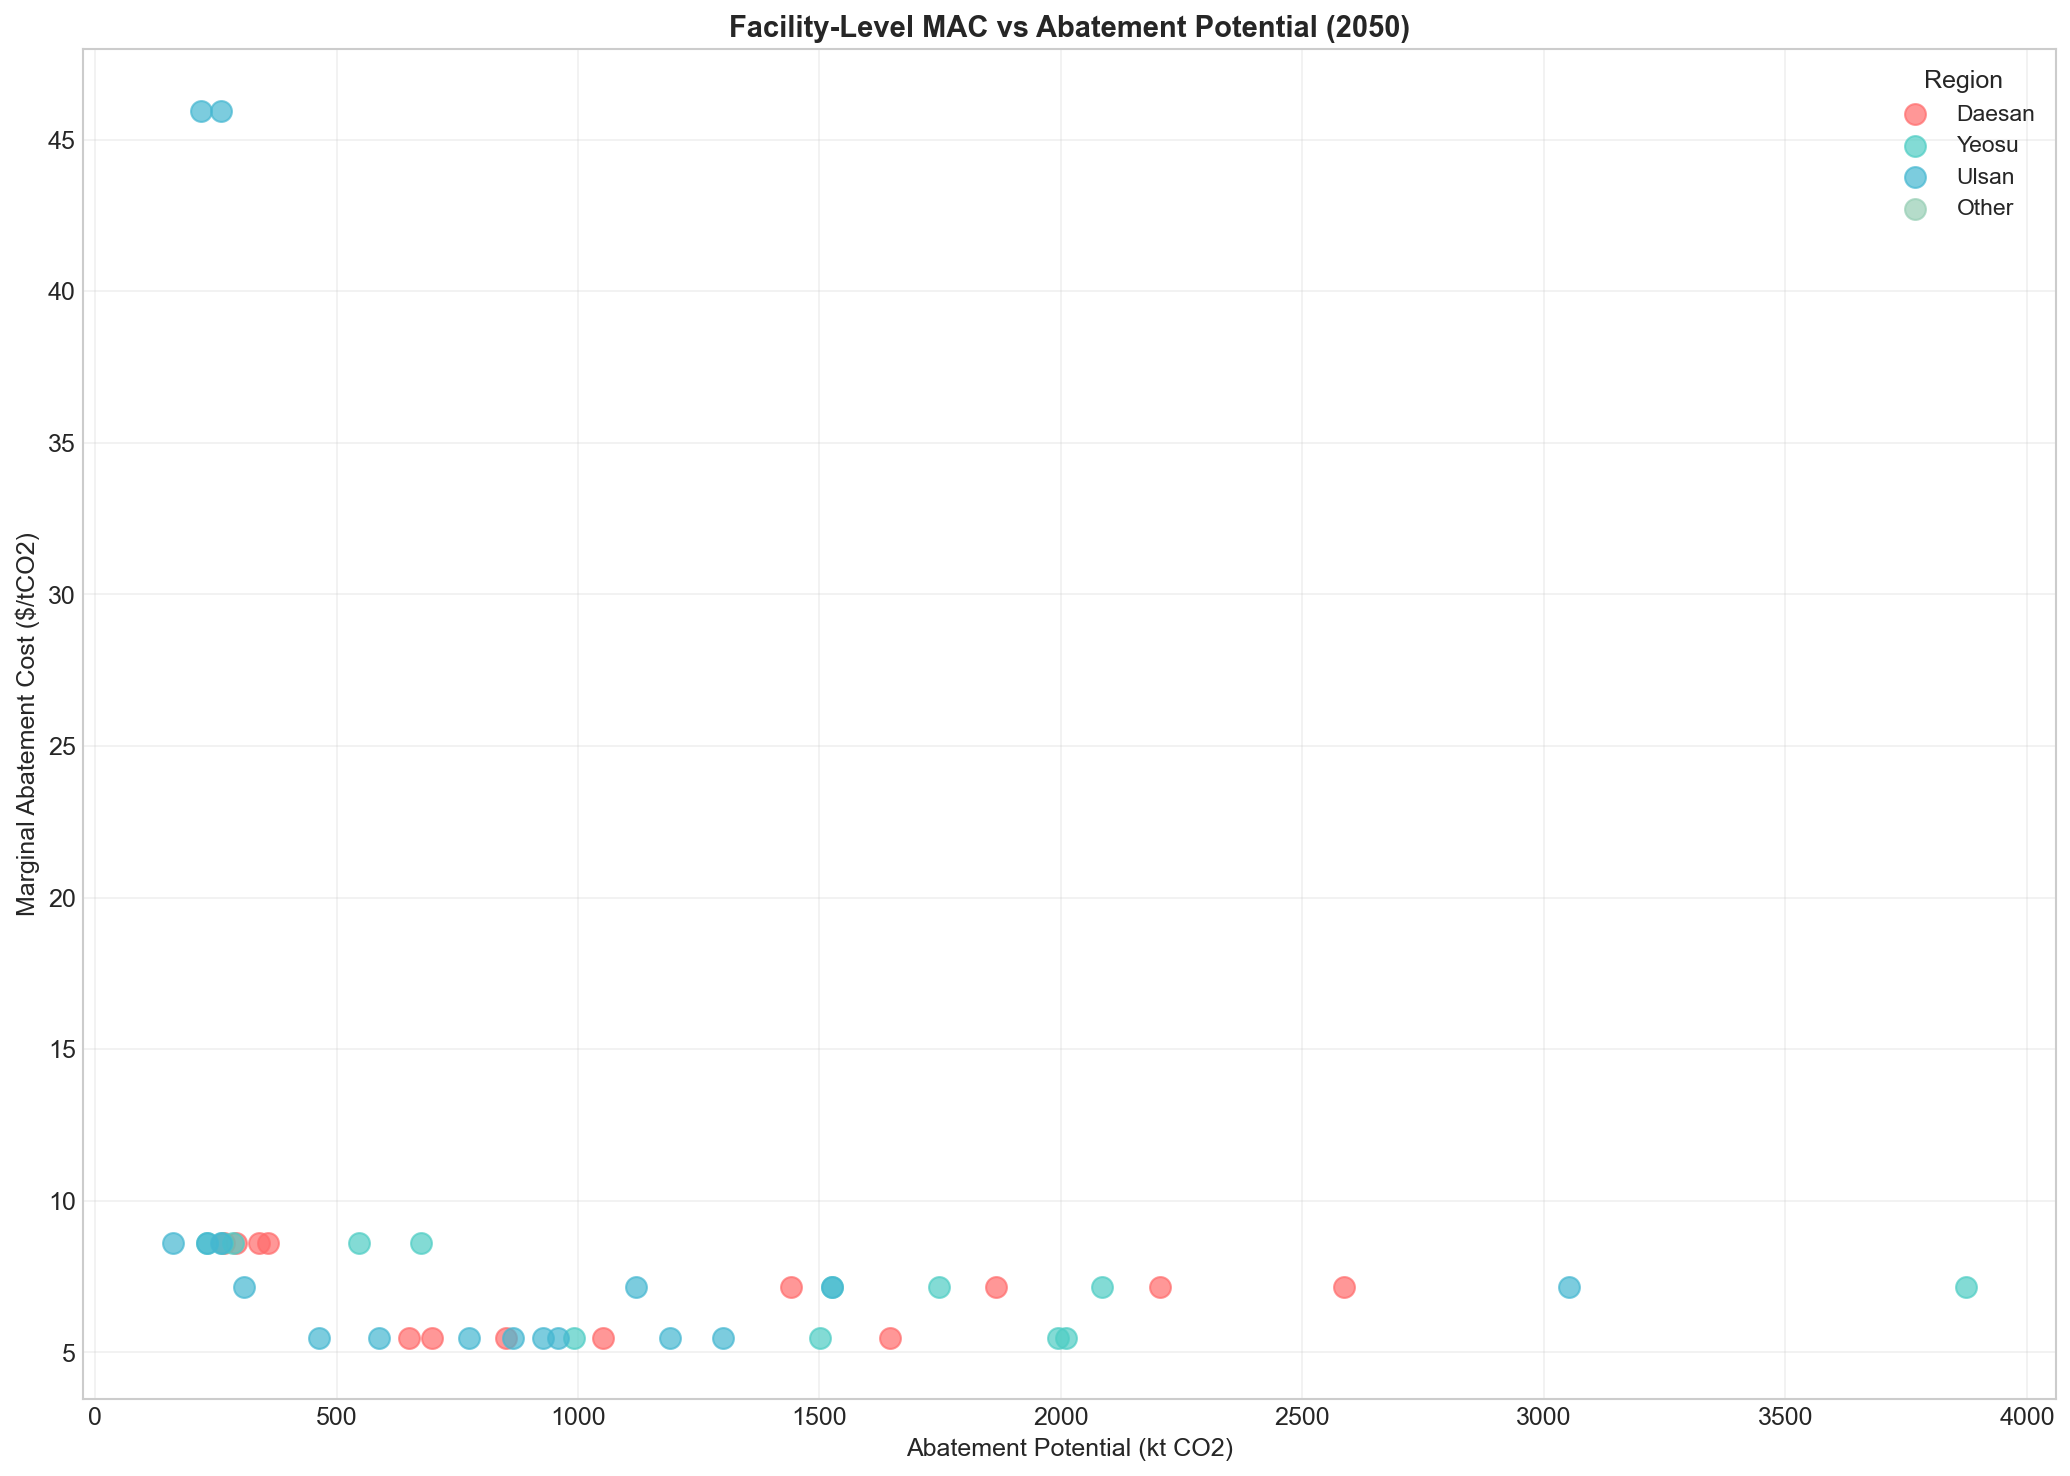
\includegraphics[width=0.95\textwidth]{../outputs/figures/report_facility_scatter.png}
\caption{Facility-level scatter plot showing MAC (\$/t~\COtwo) versus abatement potential (kt~\COtwo) for 2050 under the Shaheen NCC-H2 scenario. Points are colored by region.}
\label{fig:facility_scatter}
\end{figure}

The scatter plot reveals substantial heterogeneity in facility-level economics:
\begin{itemize}
\item MACs range from \$50 to \$500 per t~\COtwo, depending on facility characteristics and technology choice.
\item Naphtha crackers show the highest abatement potential ($>$100 kt~\COtwo/facility).
\item Yeosu facilities cluster at higher abatement potential, reflecting the complex's scale.
\item Ulsan facilities show greater cost variation, potentially due to facility age differences.
\end{itemize}

\subsection{Cumulative Investment Requirements}

Table~\ref{tab:investment} presents the cumulative investment requirements across scenarios.

\begin{table}[H]
\centering
\caption{Cumulative Investment Requirements (2025--2050)}
\label{tab:investment}
\begin{tabular}{@{}lrrr@{}}
\toprule
\textbf{Scenario} & \textbf{Cum. CAPEX} & \textbf{Est. OPEX}$^*$ & \textbf{Net Total Cost} \\
 & (\$B) & (\$B) & (\$B) \\
\midrule
shaheen\_ncc\_h2 & 825.87 & 165.17 & 80.04 \\
shaheen\_ncc\_elec & 1,242.06 & 248.41 & $-$61.22 \\
restructure\_25pct\_ncc\_h2 & 157.68 & 31.54 & 5.99 \\
restructure\_25pct\_ncc\_elec & 160.34 & 32.07 & $-$19.89 \\
restructure\_40pct\_ncc\_h2 & 113.47 & 22.69 & 3.56 \\
restructure\_40pct\_ncc\_elec & 115.45 & 23.09 & $-$15.00 \\
\bottomrule
\multicolumn{4}{l}{\footnotesize $^*$Estimated at 20\% of cumulative CAPEX.}
\end{tabular}
\end{table}

Negative net total costs for electric scenarios indicate that fuel savings exceed new energy costs over the analysis period, though this assumes continued fossil fuel price trajectories and does not account for potential carbon pricing.

%%%%%%%%%%%%%%%%%%%%%%%%%%%%%%%%%%%%%%%%%%%%%%%%%%%%%%%%%%%%%%%%%%%%%%%%%%%%%%%
%% 7. Discussion
%%%%%%%%%%%%%%%%%%%%%%%%%%%%%%%%%%%%%%%%%%%%%%%%%%%%%%%%%%%%%%%%%%%%%%%%%%%%%%%
\section{Discussion}

\subsection{Policy Implications}

The analysis yields several policy-relevant insights:

\textbf{Production Pathway Dominance:} The choice between capacity growth and restructuring has a more significant impact on transition costs than technology selection. Restructuring scenarios reduce cumulative CAPEX by 85--91\%, suggesting that capacity rationalization should be prioritized in policy design.

\textbf{Technology Selection Trade-offs:} H2-based pathways offer lower cumulative CAPEX but require substantial hydrogen infrastructure investment not captured in facility-level costs. Electric pathways have higher CAPEX but may achieve negative net operating costs and leverage existing grid infrastructure.

\textbf{Carbon Budget Alignment:} The 1.5°C pathway is structurally challenging because NCC technologies (addressing 70\%+ of emissions) are unavailable until 2030, while the pathway requires net-zero by 2035. Policy should consider aligning targets with the 2.0°C pathway while supporting accelerated technology development.

\subsection{Infrastructure Requirements}

Table~\ref{tab:infrastructure} presents the renewable energy infrastructure requirements implied by each scenario.

\begin{table}[H]
\centering
\caption{Renewable Energy Infrastructure Requirements (2050)}
\label{tab:infrastructure}
\begin{tabular}{@{}lrrr@{}}
\toprule
\textbf{Scenario} & \textbf{Electricity} & \textbf{RE Capacity}$^*$ & \textbf{Electrolyzer}$^\dagger$ \\
 & (TWh) & (GW) & (GW) \\
\midrule
shaheen\_ncc\_h2 & 166.43 & 47.6 & 85.6 \\
shaheen\_ncc\_elec & 273.58 & 78.2 & --- \\
restructure\_25pct\_ncc\_h2 & 18.49 & 5.3 & 46.6 \\
restructure\_25pct\_ncc\_elec & 76.89 & 22.0 & --- \\
restructure\_40pct\_ncc\_h2 & 40.97 & 11.7 & 40.5 \\
restructure\_40pct\_ncc\_elec & 93.32 & 26.7 & --- \\
\bottomrule
\multicolumn{4}{l}{\footnotesize $^*$Assuming 40\% capacity factor. $^\dagger$Assuming 50 kg H$_2$/kW/year.}
\end{tabular}
\end{table}

The infrastructure requirements span a wide range: 5--78 GW of additional renewable capacity and 40--86 GW of electrolyzer capacity for H2 scenarios. These requirements represent significant additions to Korea's current power system and would require coordinated infrastructure planning.

\subsection{Sensitivity Analysis}

Figure~\ref{fig:sensitivity} presents the sensitivity of stranded asset values to key assumptions.

\begin{figure}[H]
\centering
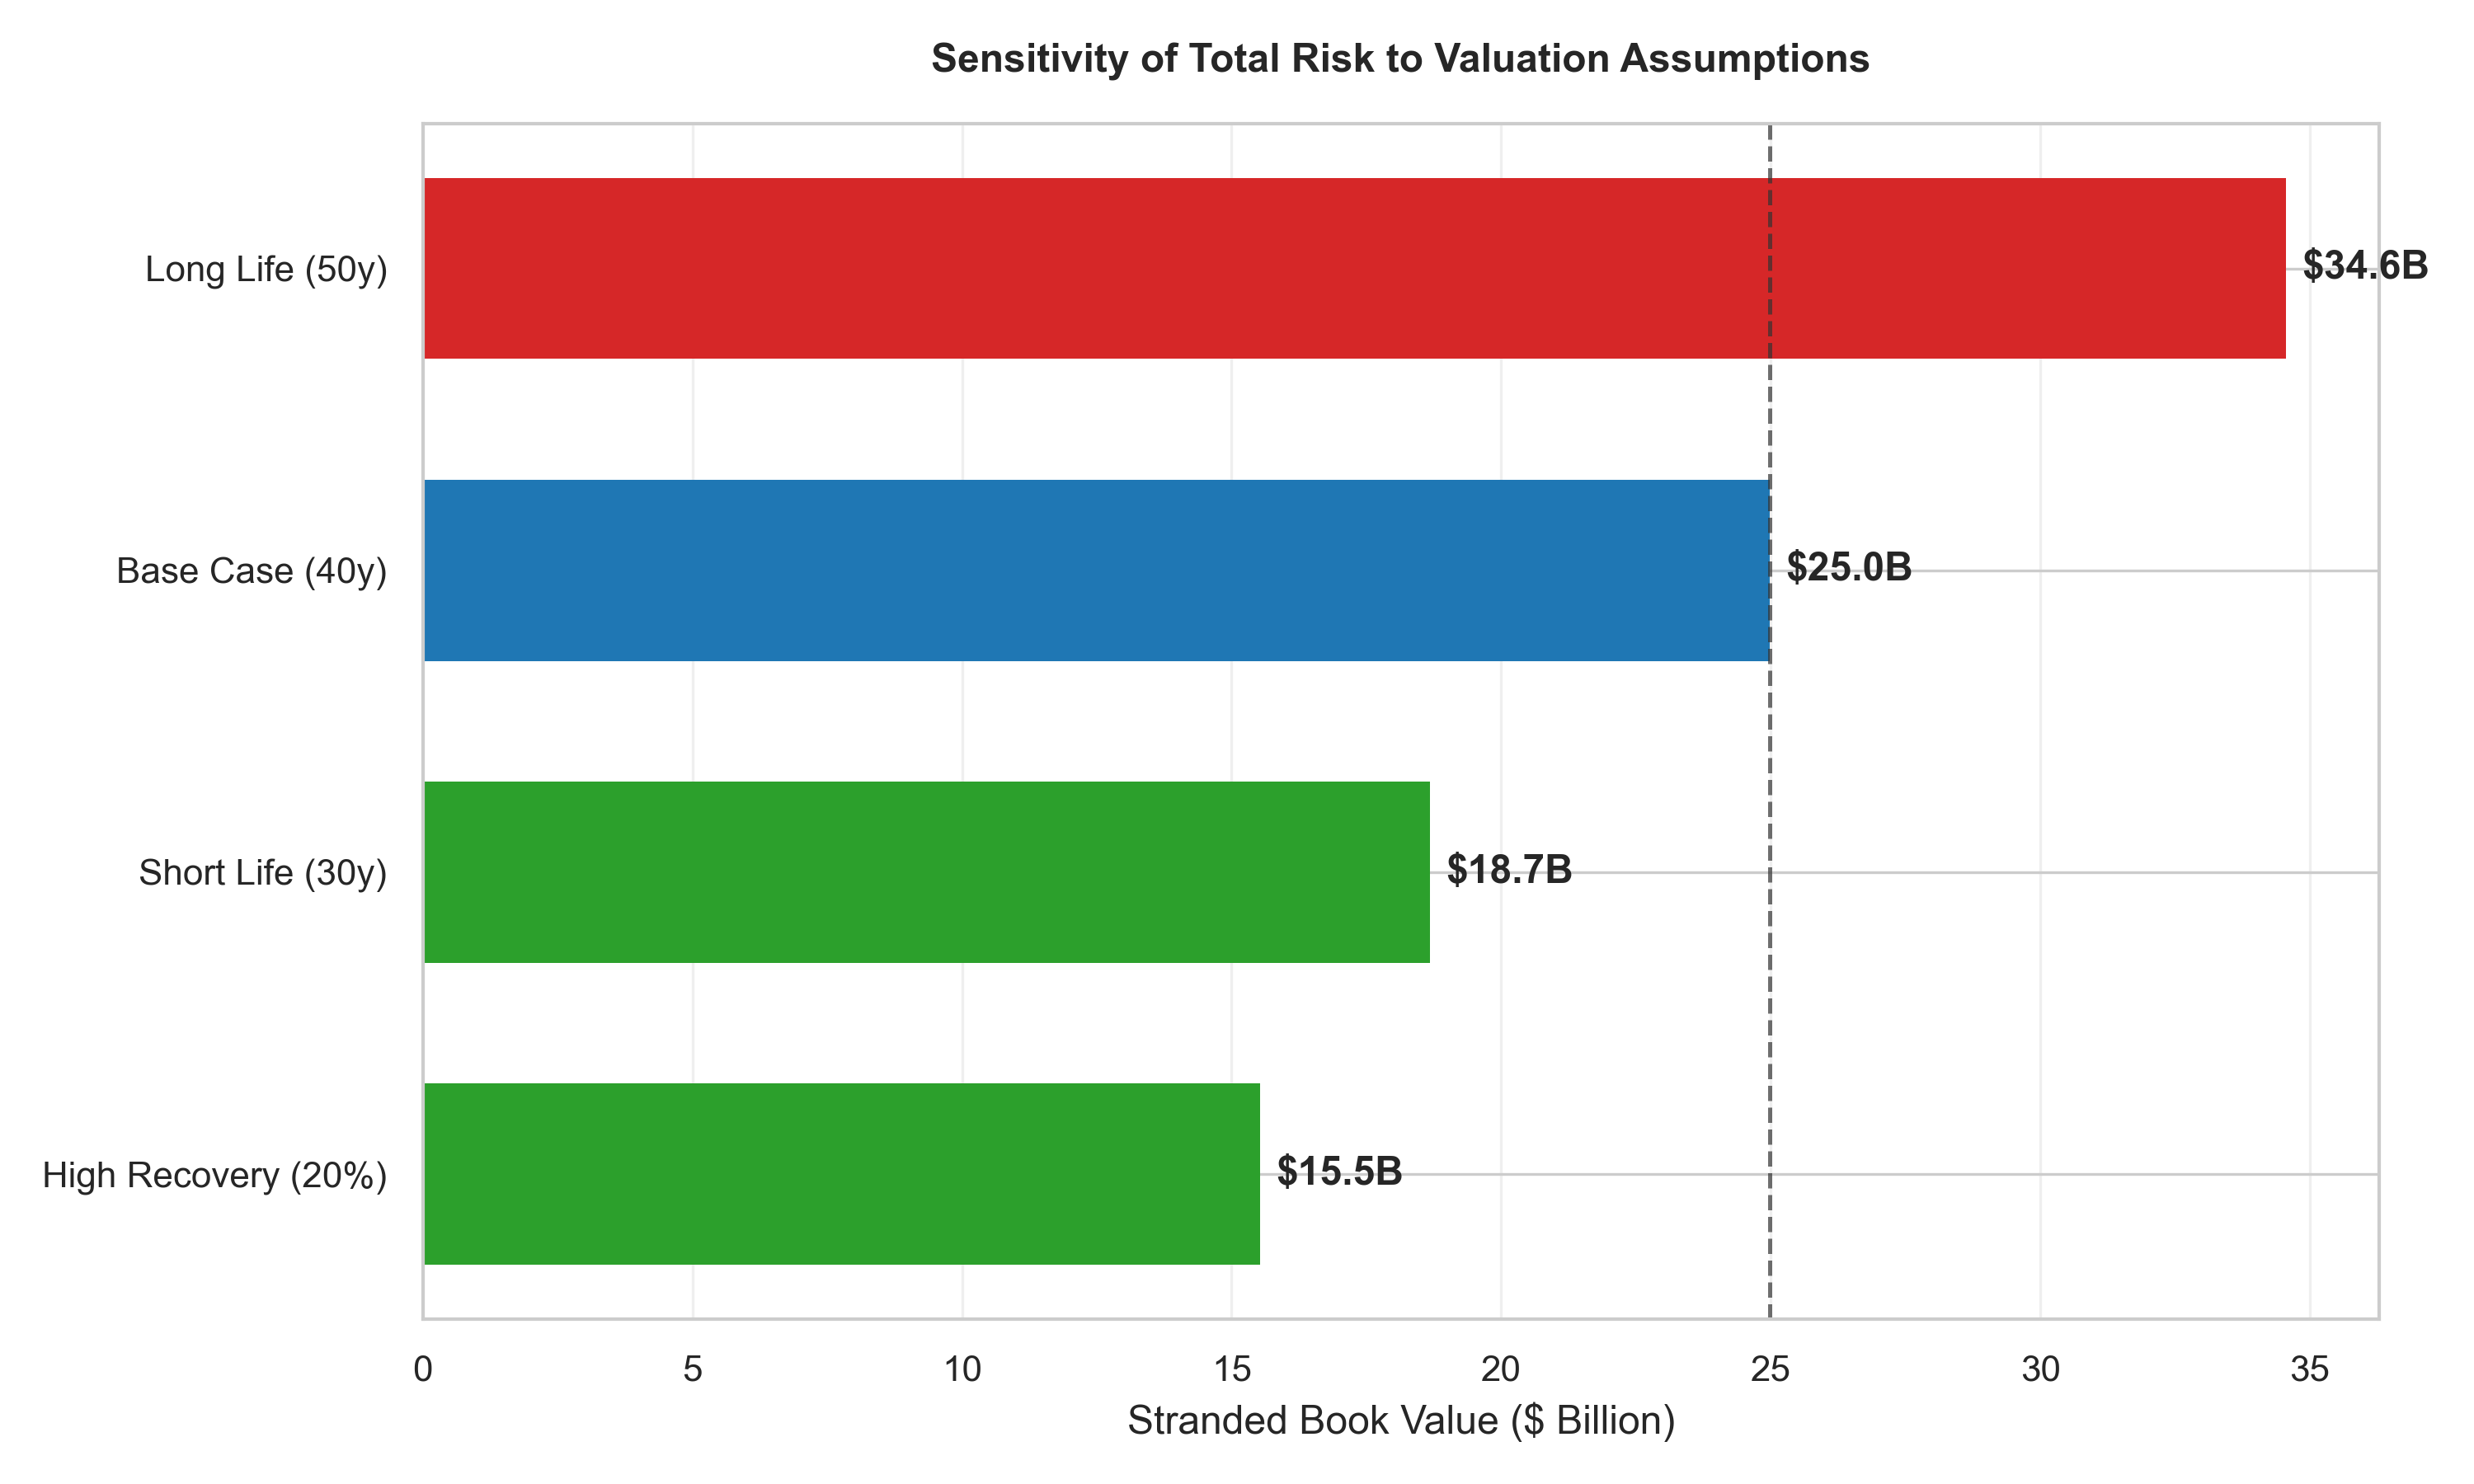
\includegraphics[width=0.85\textwidth]{../outputs/figures/sensitivity_tornado.png}
\caption{Sensitivity tornado diagram showing the impact of asset lifetime (30--50 years) and recovery rate (0--20\%) assumptions on stranded asset valuation.}
\label{fig:sensitivity}
\end{figure}

\subsection{Limitations}

This analysis has several limitations:

\begin{enumerate}
\item \textbf{Feedstock Alternatives:} The analysis does not consider potential demand shifts to bio-based or recycled feedstocks, which could reduce both production volumes and emission intensities.

\item \textbf{Technology Learning:} CAPEX reduction trajectories assume continuous learning curve effects; actual cost reductions may be discontinuous or slower.

\item \textbf{Grid Integration:} The analysis assumes grid emission factors follow government projections; actual decarbonization may vary based on policy implementation and renewable deployment pace.

\item \textbf{Infrastructure Constraints:} Regional grid constraints, hydrogen transport infrastructure, and storage requirements are not explicitly modeled.

\item \textbf{Demand Elasticity:} Production levels are assumed fixed within scenarios; price-induced demand changes are not considered.
\end{enumerate}

%%%%%%%%%%%%%%%%%%%%%%%%%%%%%%%%%%%%%%%%%%%%%%%%%%%%%%%%%%%%%%%%%%%%%%%%%%%%%%%
%% 8. Conclusion
%%%%%%%%%%%%%%%%%%%%%%%%%%%%%%%%%%%%%%%%%%%%%%%%%%%%%%%%%%%%%%%%%%%%%%%%%%%%%%%
\section{Conclusion}

This study presents a comprehensive facility-level analysis of decarbonization pathways for Korea's petrochemical industry. The key conclusions are:

\begin{enumerate}
\item \textbf{Technical Feasibility:} All six scenarios achieve net-zero emissions by 2050 through optimized deployment of available technologies (heat pumps, RDH, NCC-H2, NCC-Electricity).

\item \textbf{Restructuring Benefits:} Production pathway choices dominate cost outcomes. Restructuring scenarios that retire 25--40\% of oldest NCC capacity reduce cumulative CAPEX by 85--91\% compared to growth scenarios.

\item \textbf{Technology Trade-offs:} H2-based pathways show lower facility-level CAPEX (\$113--826B vs. \$115--1,242B for electric), but require substantial hydrogen infrastructure. Electric pathways may achieve negative net operating costs due to fuel savings.

\item \textbf{Stranded Asset Risk:} Under a 1.5°C-aligned carbon budget, stranded asset exposure ranges from \$14.4B to \$24.6B. The 2.0°C pathway substantially reduces this risk to \$3.45B--\$10.43B.

\item \textbf{Carbon Budget Constraints:} The 1.5°C pathway is structurally challenging because key NCC technologies are unavailable until 2030, while the pathway requires net-zero by 2035.

\item \textbf{Infrastructure Scale:} Achieving net-zero requires 5--85 GW of additional renewable/electrolyzer capacity, depending on scenario and technology choice.
\end{enumerate}

Policy recommendations include: (1) prioritizing 25--40\% capacity restructuring to manage transition costs; (2) developing dedicated hydrogen infrastructure if the H2 pathway is selected; (3) aligning carbon pricing with the 2.0°C pathway given technology constraints; and (4) coordinating renewable energy deployment to meet petrochemical sector needs.

Future research should address feedstock diversification options, regional grid integration constraints, and the interaction between petrochemical decarbonization and broader industrial policy.

%%%%%%%%%%%%%%%%%%%%%%%%%%%%%%%%%%%%%%%%%%%%%%%%%%%%%%%%%%%%%%%%%%%%%%%%%%%%%%%
%% Acknowledgments
%%%%%%%%%%%%%%%%%%%%%%%%%%%%%%%%%%%%%%%%%%%%%%%%%%%%%%%%%%%%%%%%%%%%%%%%%%%%%%%
\section*{Acknowledgments}

The authors thank the Korea Petrochemical Industry Association for data access and industry consultation. This research was supported by PLANiT Institute internal research funding.

\section*{Data Availability}

The facility database and model code are available from PLANiT Institute upon reasonable request for academic research purposes.

%%%%%%%%%%%%%%%%%%%%%%%%%%%%%%%%%%%%%%%%%%%%%%%%%%%%%%%%%%%%%%%%%%%%%%%%%%%%%%%
%% References
%%%%%%%%%%%%%%%%%%%%%%%%%%%%%%%%%%%%%%%%%%%%%%%%%%%%%%%%%%%%%%%%%%%%%%%%%%%%%%%
\newpage
\bibliography{references}

%%%%%%%%%%%%%%%%%%%%%%%%%%%%%%%%%%%%%%%%%%%%%%%%%%%%%%%%%%%%%%%%%%%%%%%%%%%%%%%
%% Appendices
%%%%%%%%%%%%%%%%%%%%%%%%%%%%%%%%%%%%%%%%%%%%%%%%%%%%%%%%%%%%%%%%%%%%%%%%%%%%%%%
\newpage
\appendix

\section{Complete Company Emissions List}

Table~\ref{tab:all_companies} presents the complete list of companies by baseline emissions.

\begin{longtable}{@{}clr@{}}
\caption{Complete Company Emissions List (Baseline 2025)} \label{tab:all_companies} \\
\toprule
\textbf{Rank} & \textbf{Company} & \textbf{Emissions (t~\COtwo)} \\
\midrule
\endfirsthead
\multicolumn{3}{c}{\tablename\ \thetable{} -- continued from previous page} \\
\toprule
\textbf{Rank} & \textbf{Company} & \textbf{Emissions (t~\COtwo)} \\
\midrule
\endhead
\midrule
\multicolumn{3}{r}{Continued on next page} \\
\endfoot
\bottomrule
\endlastfoot
1 & LG Chem & 14,358,266 \\
2 & Lotte Chemical & 11,197,668 \\
3 & Yeochon NCC & 8,617,271 \\
4 & Hanwha TotalEnergies & 7,440,228 \\
5 & GS Caltex & 5,190,277 \\
6 & SK Geocentric & 5,006,242 \\
7 & HD Hyundai Chemical & 4,960,305 \\
8 & Daehan Oil Chemical & 3,858,611 \\
9 & S-Oil & 2,981,254 \\
10 & Hanwha Solutions & 2,006,378 \\
11 & Kumho Petrochemical & 1,499,946 \\
12 & SK Energy & 1,191,309 \\
13 & SK Advanced & 1,152,880 \\
14 & Hyosung Chemical & 1,104,148 \\
15 & Taekwang Industrial & 1,041,685 \\
16 & HDHyundai Oilbank & 907,458 \\
17 & Hanwha Impact & 682,928 \\
18 & Samnam Petrochemical & 512,196 \\
19 & Caprolactam & 507,861 \\
20 & Korea INEOS Styrolution & 402,279 \\
& Others (41 companies) & 3,634,127 \\
\midrule
& \textbf{Total} & \textbf{78,247,366} \\
\end{longtable}

\section{Price Trajectory Assumptions}

Table~\ref{tab:price_trajectories} presents the energy price trajectories used in the analysis.

\begin{table}[H]
\centering
\caption{Energy Price Trajectory Assumptions (2025--2050)}
\label{tab:price_trajectories}
\begin{tabular}{@{}lrrrrr@{}}
\toprule
\textbf{Energy Source} & \textbf{2025} & \textbf{2030} & \textbf{2040} & \textbf{2050} & \textbf{Unit} \\
\midrule
Green Hydrogen & 4.58 & 3.91 & 2.82 & 2.01 & \$/kg \\
RE-PPA Electricity & 65.0 & 55.7 & 40.9 & 30.0 & \$/MWh \\
Grid Electricity & 100.0 & 118.3 & 163.8 & 191.4 & \$/MWh \\
Grid Emission Factor & 0.436 & 0.349 & 0.140 & 0.000 & t~\COtwo/MWh \\
Naphtha & 15.0 & 15.0 & 15.0 & 15.0 & \$/GJ \\
LNG & 12.0 & 12.0 & 12.0 & 12.0 & \$/GJ \\
\bottomrule
\end{tabular}
\end{table}

\section{Asset Valuation Parameters}

Table~\ref{tab:asset_params} presents the parameters used for stranded asset valuation.

\begin{table}[H]
\centering
\caption{Asset Valuation Parameters by Process Type}
\label{tab:asset_params}
\begin{tabular}{@{}lrrr@{}}
\toprule
\textbf{Process Type} & \textbf{Overnight CAPEX} & \textbf{Useful Life} & \textbf{Discount Rate} \\
 & (\$/t capacity) & (years) & (\%) \\
\midrule
Naphtha Cracker & 1,500 & 40 & 5 \\
BTX Plant & 800 & 40 & 5 \\
Utility & 500 & 30 & 5 \\
Other & 1,000 & 30 & 5 \\
\bottomrule
\end{tabular}
\end{table}

\section{Methodology Equations}

\subsection{Baseline Emissions Calculation}

For each facility $i$ with product $p$ and fuel $f$:

\begin{equation}
E_{i,\text{baseline}} = \sum_f \left( \text{Production}_i \times \text{EI}_{p,f} \times \text{EF}_f \right)
\end{equation}

where EI is energy intensity (GJ/t or kWh/t) and EF is emission factor.

\subsection{Technology Deployment Optimization}

The model deploys technologies in order of ascending LCOA until the emission target is met:

\begin{equation}
\min \sum_{i,t} \text{LCOA}_{i,t} \times x_{i,t}
\end{equation}

subject to:

\begin{align}
\sum_i E_{i,t}(1 - x_{i,t} \cdot \text{abatement rate}) &\leq \text{Budget}_t \\
x_{i,t} &\in \{0, 1\} \\
x_{i,t} &\leq \text{TechAvailable}_{i,t}
\end{align}

where $x_{i,t}$ is the binary deployment decision for facility $i$ in year $t$.

%%%%%%%%%%%%%%%%%%%%%%%%%%%%%%%%%%%%%%%%%%%%%%%%%%%%%%%%%%%%%%%%%%%%%%%%%%%%%%%
\end{document}
